\documentclass[dvipdfmx]{beamer}
\usepackage{bxdpx-beamer}% dvipdfmxなので必要
\usepackage{pxjahyper}% 日本語で'しおり'したい
%\usepackage{etex}
%\usetheme{Warsaw}
\usetheme{Malmoe}
%\usetheme{AnnArbor}
%\usetheme{Hannover}
%\usetheme{Bergen}
%\usetheme{Berlin}
%\usetheme{Singapore}
%\usetheme{Montpellier}
%\usetheme{Pittsburgh}
\usepackage{graphicx}
\usepackage{latexsym,amssymb}
\usepackage{amsthm}
%\usepackage{epsbox}
%\usepackage{multirow}
\usepackage{fancybox}
\usepackage{ascmac}
\usepackage{fancyvrb}
%\usepackage{listings}
\usepackage{tabularx}
\usepackage{tikz}
\usetikzlibrary{calc,shapes}
\usepackage{algorithm}
\usepackage{algpseudocode}
%\usepackage{pstricks,pst-node,pst-tree}
%\usepackage{multimedia}
%\usepackage{pstricks,pst-node,pst-tree}
%\usepackage{pst-all}
%\include{prooftree}
%\lstloadlanguages{pascal}
\usepackage{mathrsfs}

\renewcommand{\kanjifamilydefault}{\gtdefault}
\renewcommand{\familydefault}{\sfdefault}

\graphicspath{{figs261113/}}

%\include{cmacros}

\newcommand{\greentext}[1]{{\color[rgb]{0,0.5,0}{#1}}}
\newcommand{\redtext}[1]{{\color[rgb]{0.8,0,0}{#1}}}
\newcommand{\bluetext}[1]{{\color[rgb]{0,0,0.8}{#1}}}

\newcommand{\tuple}[1]{\langle{#1}\rangle}

\newcommand{\First}{\mathsf{First}_1}
\newcommand{\Follow}{\mathsf{Follow}_1}

%%pdt simulation

\newcommand{\pdtline}[6]{%
    \uncover<#6->{
    \node at (${#5}*(0,-.3)+(0,.3)$) {$\vdash$};%
    \node at (${#5}*(0,-.3)+(1.5,.3)$) {\parbox{12em}{(#1,}};%
    \node at (${#5}*(0,-.3)+(4.5,.3)$) {\parbox{10em}{#2,}};%
    \node at (${#5}*(0,-.3)+(5.7,.3)$) {\parbox{10em}{#3)}};%
    \node at (${#5}*(0,-.3)+(8,.3)$) {\parbox{20em}{#4}};%
    }
}

\newcommand{\initpdtline}[6]{%
    \uncover<#6->{
    \node at (${#5}*(0,-.3)+(1.5,.3)$) {\parbox{12em}{(#1,}};%
    \node at (${#5}*(0,-.3)+(4.5,.3)$) {\parbox{10em}{#2,}};%
    \node at (${#5}*(0,-.3)+(5.7,.3)$) {\parbox{10em}{#3)}};%
    \node at (${#5}*(0,-.3)+(8,.3)$) {\parbox{20em}{#4}};%
    }
}

\newtheorem{Def}{定義}
\newtheorem{Lem}{補題}
\newtheorem{Thm}{定理}
\newtheorem{Prop}{命題}

\newenvironment{CustomDef}[2]{%
  \par\medskip\noindent
  \textbf{定義 #1}({#2})\quad\ignorespaces
}{%
  \par\medskip
}


\definecolor{lightlightgrey}{rgb}{0.95,0.95,0.95}

\newcommand{\vdom}{\underline{\gg}}
\newcommand{\svdom}{\gg}
\newcommand{\domll}{\underline{\ll}}
\newcommand{\domv}[1]{\mathsf{dom}({#1})}
\newcommand{\idomv}[1]{\mathsf{idom}({#1})}

%\newcommand{\greentext}[1]{{\color[rgb]{0,0.5,0}{#1}}}
%\newcommand{\redtext}[1]{{\color[rgb]{0.8,0,0}{#1}}}

\newcommand{\lecturedate}{2026/11/13}

\cornersize{0.25}

\setbeamertemplate{frametitle}[default][center]
\setbeamertemplate{footline}{\hfill
コンパイラ\quad\lecturedate
\hfill\insertframenumber/\inserttotalframenumber\hspace*{1zw}}
\newcounter{coffee}
\setbeamercovered{transparent=10}
\title{コンパイラ(12)}
\date{\lecturedate}
\begin{document}

\frame{\titlepage}

\section{最適化}

\subsection{支配木}

\begin{frame}{フローグラフ$\rightarrow$支配木}
  \begin{tabular}{cc}
    \begin{minipage}{.4\textwidth}
      \scalebox{0.6}{
        \begin{tikzpicture}
          \node[anchor=west,draw,minimum width=3.8cm] (v0) at (0,6)
          {\small $\begin{array}{ll}\hspace*{1zw} & \mathtt{i=1}                               \\[-2pt]
                               & \mathtt{j=1}                               \\[-2pt]
                               & \mathtt{k=1}                               \\[-2pt]
                               & \mathtt{if}\ p\ \mathtt{goto}\ \mathtt{l1} \\\end{array}$};
          \node at ($(v0)+(-2.2,0.7)$) {$v_0$};
          \node[anchor=west,draw,minimum width=3.8cm] (v1) at (0,4)
          {\small $\begin{array}{ll}
                L3: & \mathtt{if}\ q\ \mathtt{goto}\ \mathtt{L2} \\
              \end{array}$};
          \node at ($(v1)+(-2.2,0)$) {$v_1$};
          \node[anchor=west,draw,minimum width=3.8cm] (v2) at (0,2.5)
          {\small $\begin{array}{ll}
                \hspace*{1zw} & \mathtt{i=i+1}   \\
                              & \mathtt{goto L3}
              \end{array}$};
          \node at ($(v2)+(-2.2,0.2)$) {$v_2$};
          \node[anchor=west,draw,minimum width=3.8cm] (v3) at (0,1)
          {\small $\begin{array}{ll}
                L1: & \mathtt{j=i+k} \\
              \end{array}$};
          \node at ($(v3)+(-2.2,0)$) {$v_3$};
          \node[anchor=west,draw,minimum width=3.8cm] (v4) at (0,0)
          {\small $\begin{array}{ll}
                L2: & \mathtt{k=i+j} \\
              \end{array}$};
          \node at ($(v4)+(-2.2,0)$) {$v_4$};
          \path[->] (v0) edge (v1);
          \path[->] (v1) edge (v2);
          \path[->] (v2) [out=210,in=150,looseness=3] edge (v1);
          \path[->] (v0) [out=350,in=10,looseness=0.5] edge (v3);
          \path[->] (v1) [out=350,in=10,looseness=0.5] edge (v4);
        \end{tikzpicture}
      }
    \end{minipage}
     &
    \begin{minipage}{.5\textwidth}
      \scalebox{0.6}{
        \begin{tikzpicture}
          \node[draw,circle] (v0) at (0,3) {$v_0$};
          \node[draw,circle] (v1) at (0,1.5) {$v_1$};
          \node[draw,circle] (v2) at (0,0) {$v_2$};
          \node[draw,circle] (v3) at (1.5,1.5) {$v_3$};
          \node[draw,circle] (v4) at (1.5,0) {$v_4$};
          \path[->] (v0) edge (v1)  (v0) edge (v3)  (v1) edge (v2)  (v1) edge (v4) (v3) edge (v4) (v2) [out=225,in=135] edge (v1);
          \node at (0.75,-1) {\small フローグラフ};

          \node[draw,circle] (w0) at (4.5,3) {$v_0$};
          \node[draw,circle] (w1) at (3,1.5) {$v_1$};
          \node[draw,circle] (w2) at (3,0) {$v_2$};
          \node[draw,circle] (w3) at (4.5,1.5) {$v_3$};
          \node[draw,circle] (w4) at (6,1.5) {$v_4$};
          \path[->] (w0) edge (w1) (w0) edge (w3) (w0) edge (w4) (w1) edge (w2);
          \node at (4.5,-1) {\small 支配木};
        \end{tikzpicture}
      }
    \end{minipage}
  \end{tabular}
\end{frame}

\subsection{SSA}

\begin{frame}
  \frametitle{静的単一代入を用いた最適化}

  データフロー解析のもうひとつの手法:\\
  静的単一代入(Static Single Assignment:SSA)\\
  \redtext{各変数の定義がプログラム中で唯一}

  二度目の代入が発生すると変数名を変更\\
  % \quad\greentext{変数を見ればUdチェーンがすぐに判明する。}\\
  \quad\greentext{値が同じの共通部分式が判別できる=式として一致}

  %  変換例：例6.20、6.21\\
  定義ごとに変数に添字をつける。合流する場合は、$\varphi$関数で表現

  いかにして、SSA形式を得るか？

  \vspace*{5pt}

  \begin{list}{}{}
    \item [(1)] $\varphi$関数の挿入
    \item [(2)] 変数の添字の決定
  \end{list}
  \par\vspace*{3pt}\par
  \qquad\redtext{SSA形式において最適化}
  \par\vspace*{3pt}\par
  \begin{list}{}{}
    \item [(3)] SSAから逆変換する。($\varphi$関数の消去)
  \end{list}

  \greentext{近年のコンパイラでよく用いられる手法}

\end{frame}

\begin{frame}
  \frametitle{例}

  \begin{center}
    \begin{tabular}{c}
      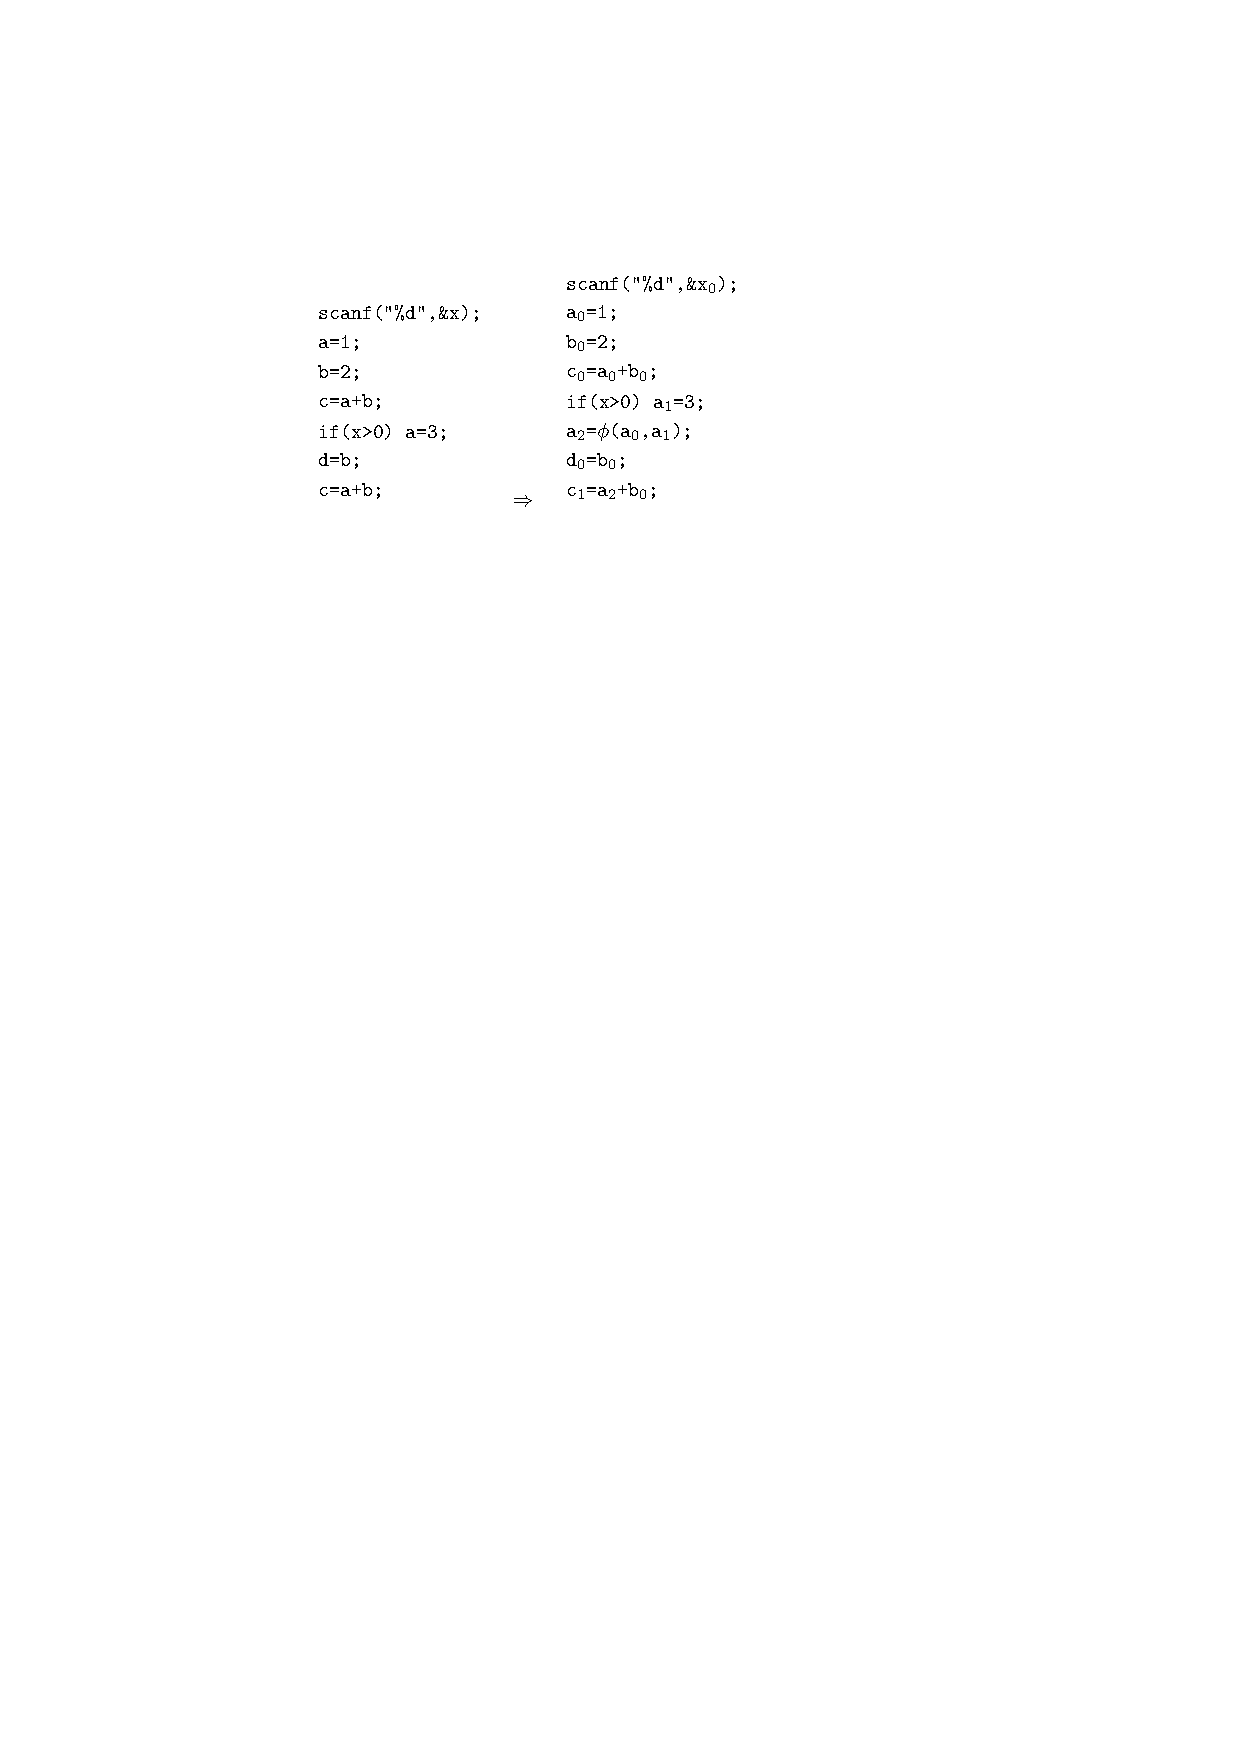
\includegraphics[height=.4\textheight]{ex6_20r1.pdf}
      \\
      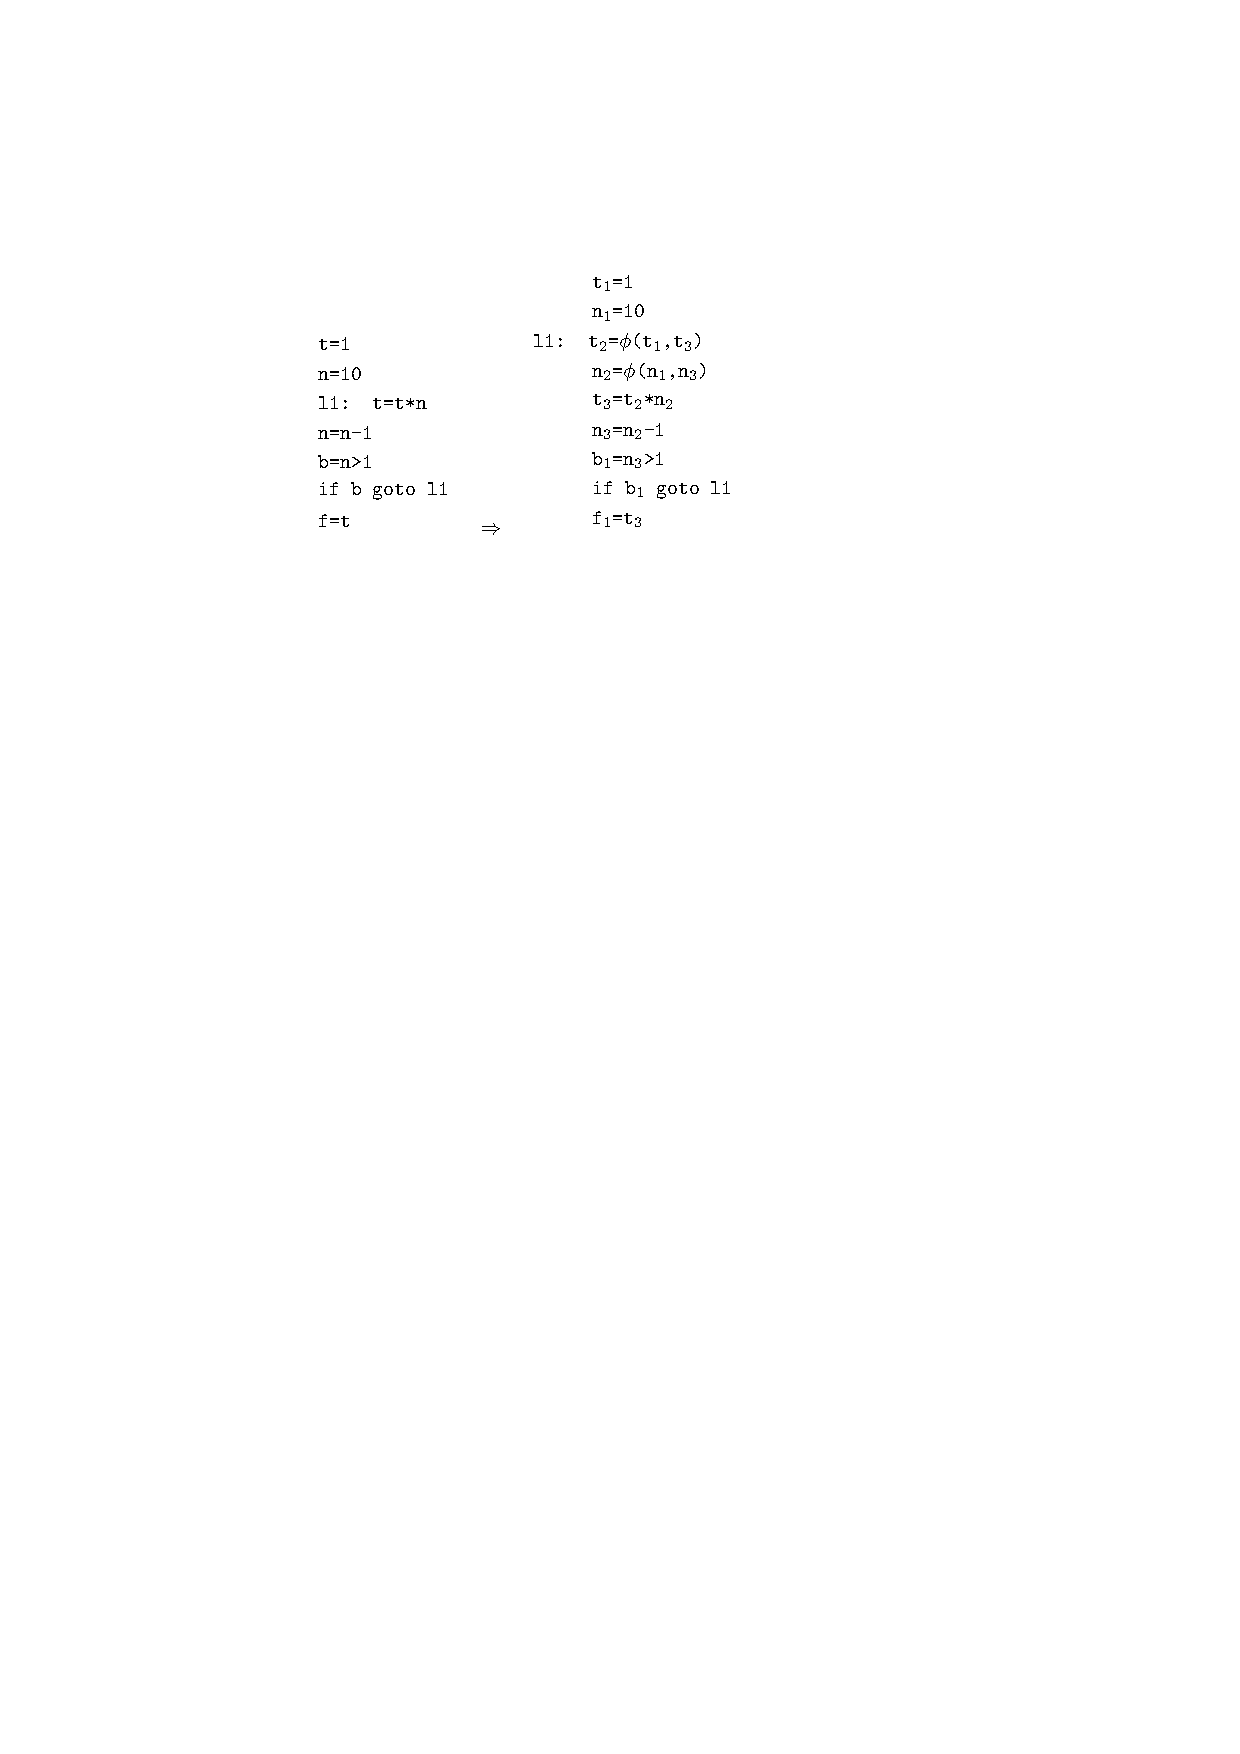
\includegraphics[height=.4\textheight]{ex6_21r1.pdf}
    \end{tabular}
  \end{center}
\end{frame}

\begin{frame}[fragile]
  \frametitle{$\varphi$関数の挿入}

%  フローグラフ：$(V,E,v_{init})$

  $\texttt{x=}\varphi(\texttt{x},\cdots,\texttt{x})$の挿入：

  \vspace*{10pt}

  \begin{quote}
    \begin{trivlist}
    \item[$\cdot$] 変数\verb|x|に対して定義7.1の条件を満たす$v_0$, $u_0$, $v$がフローグラフに存在し，頂点$v$の基本ブロックに$\varphi$関数が含まれていないならば，$v$に\verb|x=|$\varphi$\verb|(x,...,x)|を挿入する．\\[10pt]
    \item[$\cdot$] 定義合流条件を満たす$v_0$, $u_0$, $v$ がなくなるまで，上記を繰り返す．
        \end{trivlist}
  \end{quote}
\end{frame}

\begin{frame}
  \frametitle{支配辺境}

  フローグラフ$G=(V,E)$

  \begin{Def}
    $v$の支配辺境(Dominance Frontier)
    \[DF(v)=\{u\in V|\exists w.w\in
      pred(u),v\underline{\gg}w,v\not\gg u\}
    \]
  \end{Def}

  \greentext{強く支配していれば$\phi$関数を挿入する必要なし}

  \begin{center}
    \begin{tikzpicture}
      \draw[style=dashed] (0,0) rectangle (4,1);
      \node[draw,circle,minimum size=3mm] (u1) at (1,0.5) {};
      \node at (1,0.5) {\scriptsize $u_1$};
      \node[draw,circle,minimum size=3mm] (u2) at (2,0.5) {};
      \node at (2,0.5) {\scriptsize $u_2$};
      \node[draw,circle,minimum size=3mm] (u3) at (3,0.5) {};
      \node at (3,0.5) {\scriptsize $u_3$};

      \node[draw,circle,minimum size=3mm] (w1) at (1,2) {};
      \node at (1,2) {\scriptsize $w_1$};
      \node[draw,circle,minimum size=3mm] (w2) at (2,2) {};
      \node at (2,2) {\scriptsize $w_2$};
      \node[draw,circle,minimum size=3mm] (w3) at (3,2) {};
      \node at (3,2) {\scriptsize $w_3$};

      \node[draw,circle,minimum size=3mm] (v) at (2,3.5) {};
      \node at (2,3.5) {\scriptsize $v$};

      \node[fill,circle,minimum size=2mm] (p0) at (0,3) {};
      \node[fill,circle,minimum size=2mm] (p1) at (2.5,3.5) {};
      \node[fill,circle,minimum size=2mm] (p2) at (3.5,3) {};

      \path[->] (v) edge (w1) (v) edge (w2) (v) edge (w3)
      (w1) edge (u1) (w2) edge (u2) (w3) edge (u3)
      (p0) edge (u1) (p1) edge (u2) (p2) edge (u3);
    \end{tikzpicture}
  \end{center}

\end{frame}

\begin{frame}
  \frametitle{支配辺境の計算}

  フローグラフ$G=(V,E,v_{init})$

  \begin{Lem}
    \[
      DF(v)=DF_{local}(v)\cup\bigcup_{w\in Child(v)}DF_{up}(w)
    \]
    ここで、

    \[
      \begin{array}{rcl}
        DF_{local}(v) & = & \{u|v\rightarrow u,u\not\ll v\}                                \\
        \multicolumn{3}{p{.5\textwidth}}{
          \mbox{\greentext{$v$の後続頂点で}}}\\
          \multicolumn{3}{p{.5\textwidth}}{
            \mbox{\greentext{$v$を経由しない根からのフローが存在する頂点}}}
        \\[10pt]
        DF_{up}(v)  & = & \{u\in DF(v)|u\not\ll\idomv{v}\} \\
        \multicolumn{3}{p{.5\textwidth}}{
        \mbox{\greentext{$v$の親頂点からも支配されない頂点集合}}}
      \end{array}
    \]

  \end{Lem}
  アルゴリズム＝支配木の葉から$DF$を計算していく
\end{frame}

\begin{frame}
\frametitle{補題}
\begin{enumerate}
\item $DF_{local}(v)=\{u|v\rightarrow u, \idomv{u}\not= v\}$\\[20pt]
\item $v$の子頂点$w$に対して，\\[5pt]
$DF_{up}(w)=\{u\in DF(w)|\idomv{u}\not= v\}$
\end{enumerate}
\end{frame}

\begin{frame}
  \frametitle{支配辺境の計算アルゴリズム}

  {\small
        \begin{algorithmic}
            % \caption{支配辺境の計算}\label{alg:dominanceFrontier}
            \Procedure{computeDF}{$n$}
            \State $S \gets \{\}$
            \ForAll{$y \in \mathsf{succ}[n]$}   \Comment $DF_{local}$の計算
            \If{$\idomv{y}\not=n$}
            \State $S \gets S\cup\{y\}$
            \EndIf
            \EndFor
            \ForAll{$c \in \mathsf{Child}(n)$}  \Comment $DF_{up}$の計算
            \State computeDF(c) \Comment 支配木の子頂点から計算する
            \ForAll{$w \in DF[c]$}
            \If{$w\notin\domv{n}$ or $n=w$}
            \State $S\gets S\cup\{w\}$
            \EndIf
            \EndFor
            \EndFor
            \State $DF[n]\gets S$
            \EndProcedure
        \end{algorithmic}
  }
\end{frame}

\begin{frame}[fragile]
  \frametitle{支配辺境の計算例}
\centerline{\greentext{\small 講義ページにpythonによる実現を掲載}}
\begin{tabular}{ccc}
  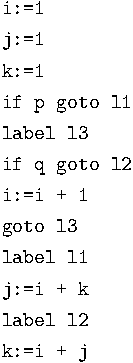
\includegraphics{7_15-prog-crop.pdf}
  &
  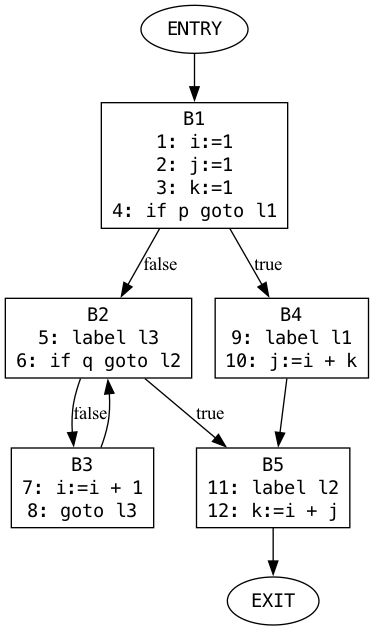
\includegraphics[scale=0.25]{ex7_15.cfg.png}
  &
  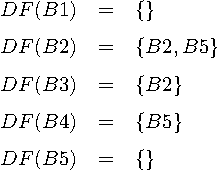
\includegraphics{7_15-DF-crop.pdf}
\end{tabular}

\end{frame}



\begin{frame}
  \frametitle{定義合流条件の計算}

  \begin{list}{}{}
    \item [定義合流条件'($S$)]
          二つのパス $p(=v_1,\cdots,v_k)$, $q(=u_1,\cdots,u_l)$
          \begin{list}{(\arabic{coffee})}{\usecounter{coffee}}
            \item $k\ge 2$, $l\ge 2$
            \item $v_1,u_1\in S$
            \item $v_k=u_l=v$
            \item $\{v_1,\cdots,v_{k-1}\}\cap\{u_1,\cdots,u_{l-1}\}=\emptyset$
          \end{list}

          \vspace*{5pt}

    \item $J(S)=\{v|\mbox{上の条件を満たす$v$}\}$
  \end{list}

  \vspace*{5pt}

  \redtext{\small
    変数$x$が定義される場所の集合を$S$とすると
    $J(S)$は、$x$に対して最初に$\phi$関数$x=\phi(x,x)$が挿入
    される場所}

  \vspace*{5pt}

  {\small\greentext{
      $\phi$関数によって新たに定義が挿入されるため、さらに挿入が必
      要:次の漸化式で不動点$J^+(S_0)$を計算}}

  \[
    \begin{array}{rcl}
      S_{i+1}      & = & J(S_0\cup S_i)                   \\
      J^{n+1}(S_0) & = & J(S_0\cup J^n(S_0))              \\
      J^+(S_0)     & = & \lim_{n\leftarrow\infty}J^n(S_0)
    \end{array}
  \]

\end{frame}

\begin{frame}
  \frametitle{支配辺境と合流条件}

  \begin{itembox}[l]{定理}
    $DF(S)=\bigcup_{v\in S}DF(v)$のとき、
    \[
      F_{i+1}=DF(S_0\cup F_i)\quad(i\ge 0,F_0=\emptyset)
    \]
    とするとき，$DF^+(S_0)=\lim_{n\leftarrow\infty}F_n$とする．
    このとき，
    \[
      DF^+(S_0)=J^+(S_0)
    \]
  \end{itembox}

  \greentext{合流条件は支配辺境から計算可能}

\end{frame}

\begin{frame}[fragile]
  \frametitle{例7.15}

  \begin{tabular}{ccc}
    \begin{minipage}{.4\textwidth}
      \scalebox{0.8}{
        \begin{tikzpicture}
          \node[anchor=west,draw,minimum width=3.8cm] (v0) at (0,6.5)
          {\small $\begin{array}{ll}\hspace*{1zw} & \mathtt{i=1}                               \\[-2pt]
                               & \mathtt{j=1}                               \\[-2pt]
                               & \mathtt{k=1}                               \\[-2pt]
                               & \mathtt{if}\ p\ \mathtt{goto}\ \mathtt{l1} \\\end{array}$};
          \node at ($(v0)+(-2.2,0.7)$) {$v_0$};
          \only<1>{\node[anchor=west,draw,minimum width=3.8cm] (v1) at (0,4.25)
            {\small $\begin{array}{ll}
                  L3: & \mathtt{if}\ q\ \mathtt{goto}\ \mathtt{L2} \\
                \end{array}$};}
          \only<2>{
            \node[anchor=west,draw,minimum width=3.8cm] (v1) at (0,4.25)
            {\small $\begin{array}{ll}
                  L3: & \mathtt{i=}\phi\mathtt{(i,i)}              \\[-2pt]
                      & \mathtt{if}\ q\ \mathtt{goto}\ \mathtt{L2} \\
                \end{array}$};}
          \node at ($(v1)+(-2.2,0)$) {$v_1$};
          \node[anchor=west,draw,minimum width=3.8cm] (v2) at (0,2.5)
          {\small $\begin{array}{ll}
                \hspace*{1zw} & \mathtt{i=i+1}   \\
                              & \mathtt{goto L3}
              \end{array}$};
          \node at ($(v2)+(-2.2,0.2)$) {$v_2$};
          \node[anchor=west,draw,minimum width=3.8cm] (v3) at (0,1)
          {\small $\begin{array}{ll}
                L1: & \mathtt{j=i+k} \\
              \end{array}$};
          \node at ($(v3)+(-2.2,0)$) {$v_3$};
          \only<1>{
            \node[anchor=west,draw,minimum width=3.8cm] (v4) at (0,-0.5)
            {\small $\begin{array}{ll}
                  L2: & \mathtt{k=i+j} \\
                \end{array}$};}
          \only<2>{
            \node[anchor=west,draw,minimum width=3.8cm] (v4) at (0,-0.5)
            {\small $\begin{array}{ll}
                  L2: & \mathtt{i=}\phi\mathtt{(i,i)} \\
                      & \mathtt{j=}\phi\mathtt{(j,j)} \\
                      & \mathtt{k=i+j}                \\
                \end{array}$};}
          \node at ($(v4)+(-2.2,0)$) {$v_4$};
          \path[->] (v0) edge (v1);
          \path[->] (v1) edge (v2);
          \path[->] (v2) [out=210,in=150,looseness=3] edge (v1);
          \path[->] (v0) [out=350,in=10,looseness=0.5] edge (v3);
          \path[->] (v1) [out=350,in=10,looseness=0.5] edge (v4);
          \path[->] (v3) edge (v4);
        \end{tikzpicture}
      }
    \end{minipage}
     & \hspace*{1zw} &
    \begin{minipage}{.5\textwidth}
      \begin{tabular}{l}
        $i$の定義：$S_0=\{v_0,v_2\}$  \\
        $j$の定義：$S'_0=\{v_0,v_3\}$ \\
        $k$の定義：$S''_0=\{v_0,v_4\}$
      \end{tabular}

      \[
        \begin{array}{l}
          DF^+(S_0)=\{v_1,v_4\} \\
          DF^+(S'_0)=\{v_4\}    \\
          DF^+(S''_0)=\emptyset
        \end{array}
      \]
    \end{minipage}
  \end{tabular}

\end{frame}

\subsection{SSA形式への変換}

\begin{frame}
\frametitle{SSA形式への変換アルゴリズム}
\begin{enumerate}
\item 各変数$x$に対してスタック$\mathsf{stack}(x)$とカウンタ$\mathsf{count}(x)$を用意して，
各スタックに$0$をプッシュして$\mathsf{count}(x)$を0に初期化

\item 支配木を深さ優先でトラバースして添字を割り当てる．
\begin{enumerate}
\item $\varphi$関数以外の右辺に各変数のスタックトップの添字を割り当て
\item スタックトップの添字を+1した数をpushして，左辺の変数にわりあて
\item $\varphi$関数の引数に先行頂点の添字のスタックトップを割り当て
\item 子頂点の添字付け
\item スタックをpopする
\end{enumerate}
\end{enumerate}

\end{frame}

\begin{frame}
  \frametitle{SSA形式への変換}
  \begin{tabular}{cc}
    \begin{minipage}{.5\textwidth}

      \scalebox{0.8}{
        \begin{tikzpicture}
          \only<1>{\node[anchor=west,draw,minimum width=3.8cm] (v0) at (0,6.5)
            {\small $\begin{array}{ll}\hspace*{1zw}
                   & \mathtt{i=1}                               \\[-2pt]
                   & \mathtt{j=1}                               \\[-2pt]
                   & \mathtt{k=1}                               \\[-2pt]
                   & \mathtt{if}\ p\ \mathtt{goto}\ \mathtt{L1} \\\end{array}$};}
          \only<2->{\node[anchor=west,draw,minimum width=3.8cm] (v0) at (0,6.5)
            {\small $\begin{array}{ll}\hspace*{1zw}
                   & \mathtt{i_1=1}                              \\[-2pt]
                   & \mathtt{j_1=1}                              \\[-2pt]
                   & \mathtt{k_1=1}                              \\[-2pt]
                   & \mathtt{if}\ p'\ \mathtt{goto}\ \mathtt{L1} \\\end{array}$};}
          \node at ($(v0)+(-2.2,0.7)$) {$v_0$};
          \only<1>{\node[anchor=west,draw,minimum width=3.8cm] (v1) at (0,4.25)
            {\small $\begin{array}{ll}
                  L3: & \mathtt{i=}\phi\mathtt{(i,i)}              \\[-2pt]
                      & \mathtt{if}\ q\ \mathtt{goto}\ \mathtt{L2} \\
                \end{array}$};}
          \only<2>{\node[anchor=west,draw,minimum width=3.8cm] (v1) at (0,4.25)
            {\small $\begin{array}{ll}
                  L3: & \mathtt{i=}\phi\mathtt{(i_1,i)}            \\[-2pt]
                      & \mathtt{if}\ q\ \mathtt{goto}\ \mathtt{L2} \\
                \end{array}$};}
          \only<3>{\node[anchor=west,draw,minimum width=3.8cm] (v1) at (0,4.25)
            {\small $\begin{array}{ll}
                  L3: & \mathtt{i_2=}\phi\mathtt{(i_1,i)}          \\[-2pt]
                      & \mathtt{if}\ q\ \mathtt{goto}\ \mathtt{L2} \\
                \end{array}$};}
          \only<4->{\node[anchor=west,draw,minimum width=3.8cm] (v1) at (0,4.25)
            {\small $\begin{array}{ll}
                  L3: & \mathtt{i_2=}\phi\mathtt{(i_1,i_3)}        \\[-2pt]
                      & \mathtt{if}\ q\ \mathtt{goto}\ \mathtt{L2} \\
                \end{array}$};}
          \node at ($(v1)+(-2.2,0)$) {$v_1$};
          \only<1-3>{\node[anchor=west,draw,minimum width=3.8cm] (v2) at (0,2.5)
            {\small $\begin{array}{ll}
                  \hspace*{1zw} & \mathtt{i=i+1}   \\
                                & \mathtt{goto L3}
                \end{array}$};}
          \only<4->{\node[anchor=west,draw,minimum width=3.8cm] (v2) at (0,2.5)
            {\small $\begin{array}{ll}
                  \hspace*{1zw} & \mathtt{i_3=i_2+1} \\
                                & \mathtt{goto L3}
                \end{array}$};}
          \node at ($(v2)+(-2.2,0.2)$) {$v_2$};
          \only<1-4>{\node[anchor=west,draw,minimum width=3.8cm] (v3) at (0,1)
            {\small $\begin{array}{ll}
                  L1: & \mathtt{j=i+k} \\
                \end{array}$};}
          \only<5->{\node[anchor=west,draw,minimum width=3.8cm] (v3) at (0,1)
            {\small $\begin{array}{ll}
                  L1: & \mathtt{j_2=i_1+k_1} \\
                \end{array}$};}
          \node at ($(v3)+(-2.2,0)$) {$v_3$};
          \only<1,2>{\node[anchor=west,draw,minimum width=3.8cm] (v4) at (0,-0.5)
            {\small $\begin{array}{ll}
                  L2: & \mathtt{i=}\phi\mathtt{(i,i)} \\
                      & \mathtt{j=}\phi\mathtt{(j,j)} \\
                      & \mathtt{k=i+j}                \\
                \end{array}$};}
          \only<3,4,5>{\node[anchor=west,draw,minimum width=3.8cm] (v4) at (0,-0.5)
            {\small $\begin{array}{ll}
                  L2: & \mathtt{i=}\phi\mathtt{(i_2,i)} \\
                      & \mathtt{j=}\phi\mathtt{(j_1,j)} \\
                      & \mathtt{k=i+j}                  \\
                \end{array}$};}
          \only<6->{\node[anchor=west,draw,minimum width=3.8cm] (v4) at (0,-0.5)
            {\small $\begin{array}{ll}
                  L2: & \mathtt{i_4=}\phi\mathtt{(i_2,i_1)} \\
                      & \mathtt{j_3=}\phi\mathtt{(j_1,j_2)} \\
                      & \mathtt{k_2=i_4+j_3}                \\
                \end{array}$};}
          \node at ($(v4)+(-2.2,0)$) {$v_4$};
          \path[->] (v0) edge (v1);
          \path[->] (v1) edge (v2);
          \path[->] (v2) [out=210,in=150,looseness=3] edge (v1);
          \path[->] (v0) [out=350,in=10,looseness=0.5] edge (v3);
          \path[->] (v1) [out=350,in=10,looseness=0.5] edge (v4);
          \path[->] (v3) edge (v4);
          \only<7>{
            \draw[color=green,line width=1.5pt] (-1.75,7.75) rectangle +(7,-9.25);
          }
        \end{tikzpicture}
      }
    \end{minipage}
     &
    \begin{minipage}{.5\textwidth}
      \begin{center}
        \begin{tikzpicture}
          \only<1-3>{\node[draw,circle,minimum size=3mm] (vt2) at (0,0) {};}
          \only<4>{\node[draw,circle,minimum size=3mm,fill=red] (vt2) at (0,0) {};}
          \only<5->{\node[draw,circle,minimum size=3mm,fill=blue] (vt2) at (0,0) {};}
          \only<1,2>{\node[draw,circle,minimum size=3mm] (vt1) at (0,1) {};}
          \only<3>{\node[draw,circle,minimum size=3mm,fill=red] (vt1) at (0,1) {};}
          \only<4->{\node[draw,circle,minimum size=3mm,fill=blue] (vt1) at (0,1) {};}
          \only<1>{\node[draw,circle,minimum size=3mm] (vt0) at (1,2) {};}
          \only<2>{\node[draw,circle,minimum size=3mm,fill=red] (vt0) at (1,2) {};}
          \only<3->{\node[draw,circle,minimum size=3mm,fill=blue] (vt0) at (1,2) {};}
          \only<1-4>{\node[draw,circle,minimum size=3mm] (vt3) at (1,1) {};}
          \only<5>{\node[draw,circle,minimum size=3mm,fill=red] (vt3) at (1,1) {};}
          \only<6->{\node[draw,circle,minimum size=3mm,fill=blue] (vt3) at (1,1) {};}
          \only<1-5>{\node[draw,circle,minimum size=3mm] (vt4) at (2,1) {};}
          \only<6->{\node[draw,circle,minimum size=3mm,fill=red] (vt4) at (2,1) {};}

          \node at (0,0) {\scriptsize $v_2$};
          \node at (0,1) {\scriptsize $v_1$};
          \node at (1,2) {\scriptsize $v_0$};
          \node at (1,1) {\scriptsize $v_3$};
          \node at (2,1) {\scriptsize $v_4$};

          \path[->] (vt0) edge (vt1) (vt0) edge (vt3) (vt0) edge (vt4) (vt1) edge (vt2);
        \end{tikzpicture}
      \end{center}
      \[
        \only<1>{\begin{array}{ll}
            stack(i)=[0] & c(i)=0 \\
            stack(j)=[0] & c(j)=0 \\
            stack(k)=[0] & c(k)=0 \\
          \end{array}}
        \only<2>{\begin{array}{ll}
            stack(i)=[1,0] & c(i)=1 \\
            stack(j)=[1,0] & c(j)=1 \\
            stack(k)=[1,0] & c(k)=1 \\
          \end{array}}
        \only<3>{\begin{array}{ll}
            stack(i)=[2,1,0] & c(i)=2 \\
            stack(j)=[1,0]   & c(j)=1 \\
            stack(k)=[1,0]   & c(k)=1 \\
          \end{array}}
        \only<4>{\begin{array}{ll}
            stack(i)=[3,2,1,0] & c(i)=3 \\
            stack(j)=[1,0]     & c(j)=1 \\
            stack(k)=[1,0]     & c(k)=1 \\
          \end{array}}
        \only<5>{\begin{array}{ll}
            stack(i)=[1,0] & c(i)=3 \\
            stack(j)=[2,1,0]   & c(j)=2 \\
            stack(k)=[1,0]     & c(k)=1 \\
          \end{array}}
        \only<6>{\begin{array}{ll}
            stack(i)=[4,1,0] & c(i)=4 \\
            stack(j)=[3,1,0]   & c(j)=3 \\
            stack(k)=[2,1,0]   & c(k)=2 \\
          \end{array}}
      \]
    \end{minipage}
  \end{tabular}
\end{frame}

\subsection{SSA形式に対する最適化}

% \begin{frame}
%   \frametitle{SSA形式に対する最適化}
%   SSA形式：データフロー解析ずみのプログラム\\[2zw]

%   \greentext{構文的にフローが表現されている}
%   $\Rightarrow$
%   \redtext{最適化を効果的に適用できる}：
%   \greentext{更新のチェックが不要}

%   例：DAGの構成が容易

%   \vspace*{1zw}

%   \begin{itemize}
%     \item 不用コードの削除
%     \item 定数伝播
%     \item コピー伝播
%     \item 共通部分式の削除
%     \item ループ不変コードの移動
%   \end{itemize}
% \end{frame}

% \begin{frame}
%   \frametitle{SSA最適化例 [佐々:06]}

%   \only<1>{
%     \begin{center}
%       \begin{tabular}{ccc}
%         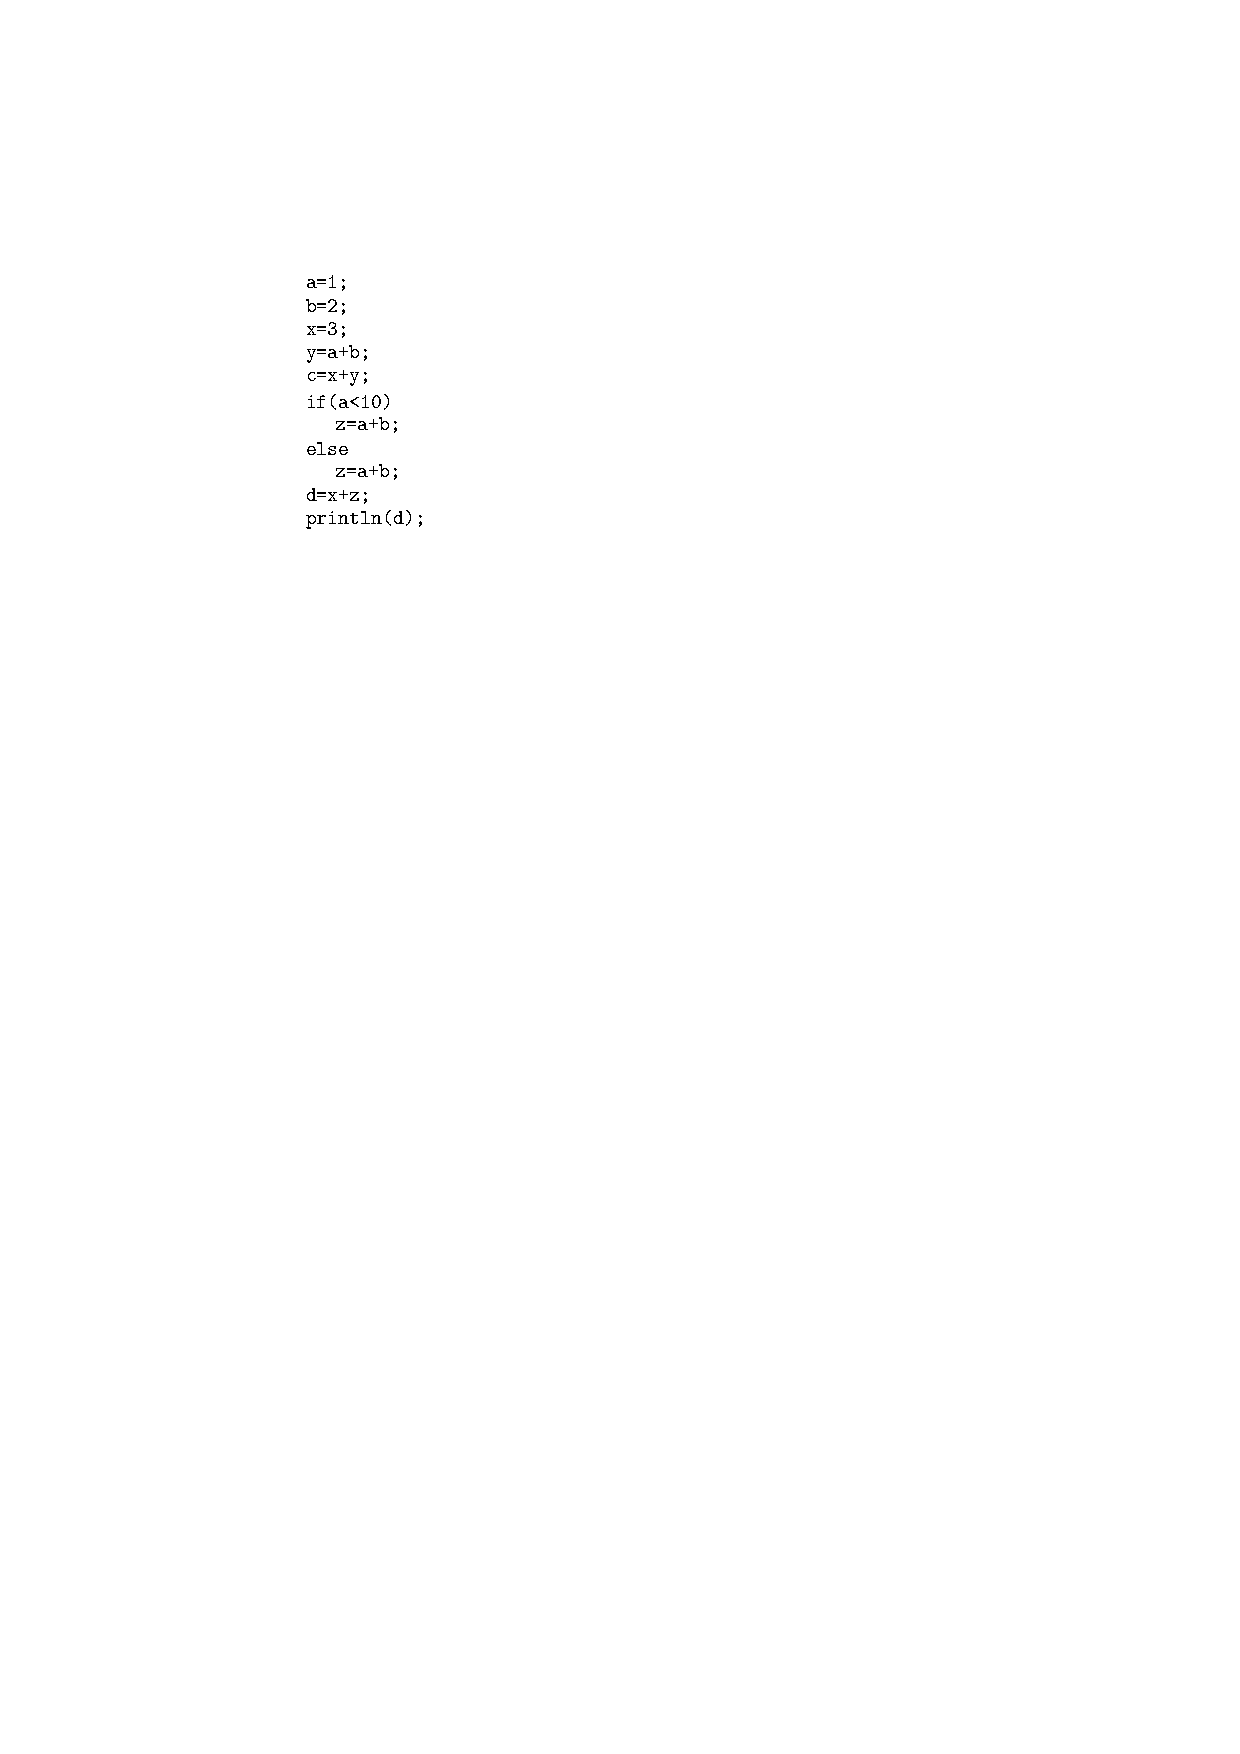
\includegraphics{ssasrc01.pdf}
%          & $\Rightarrow$ &
%         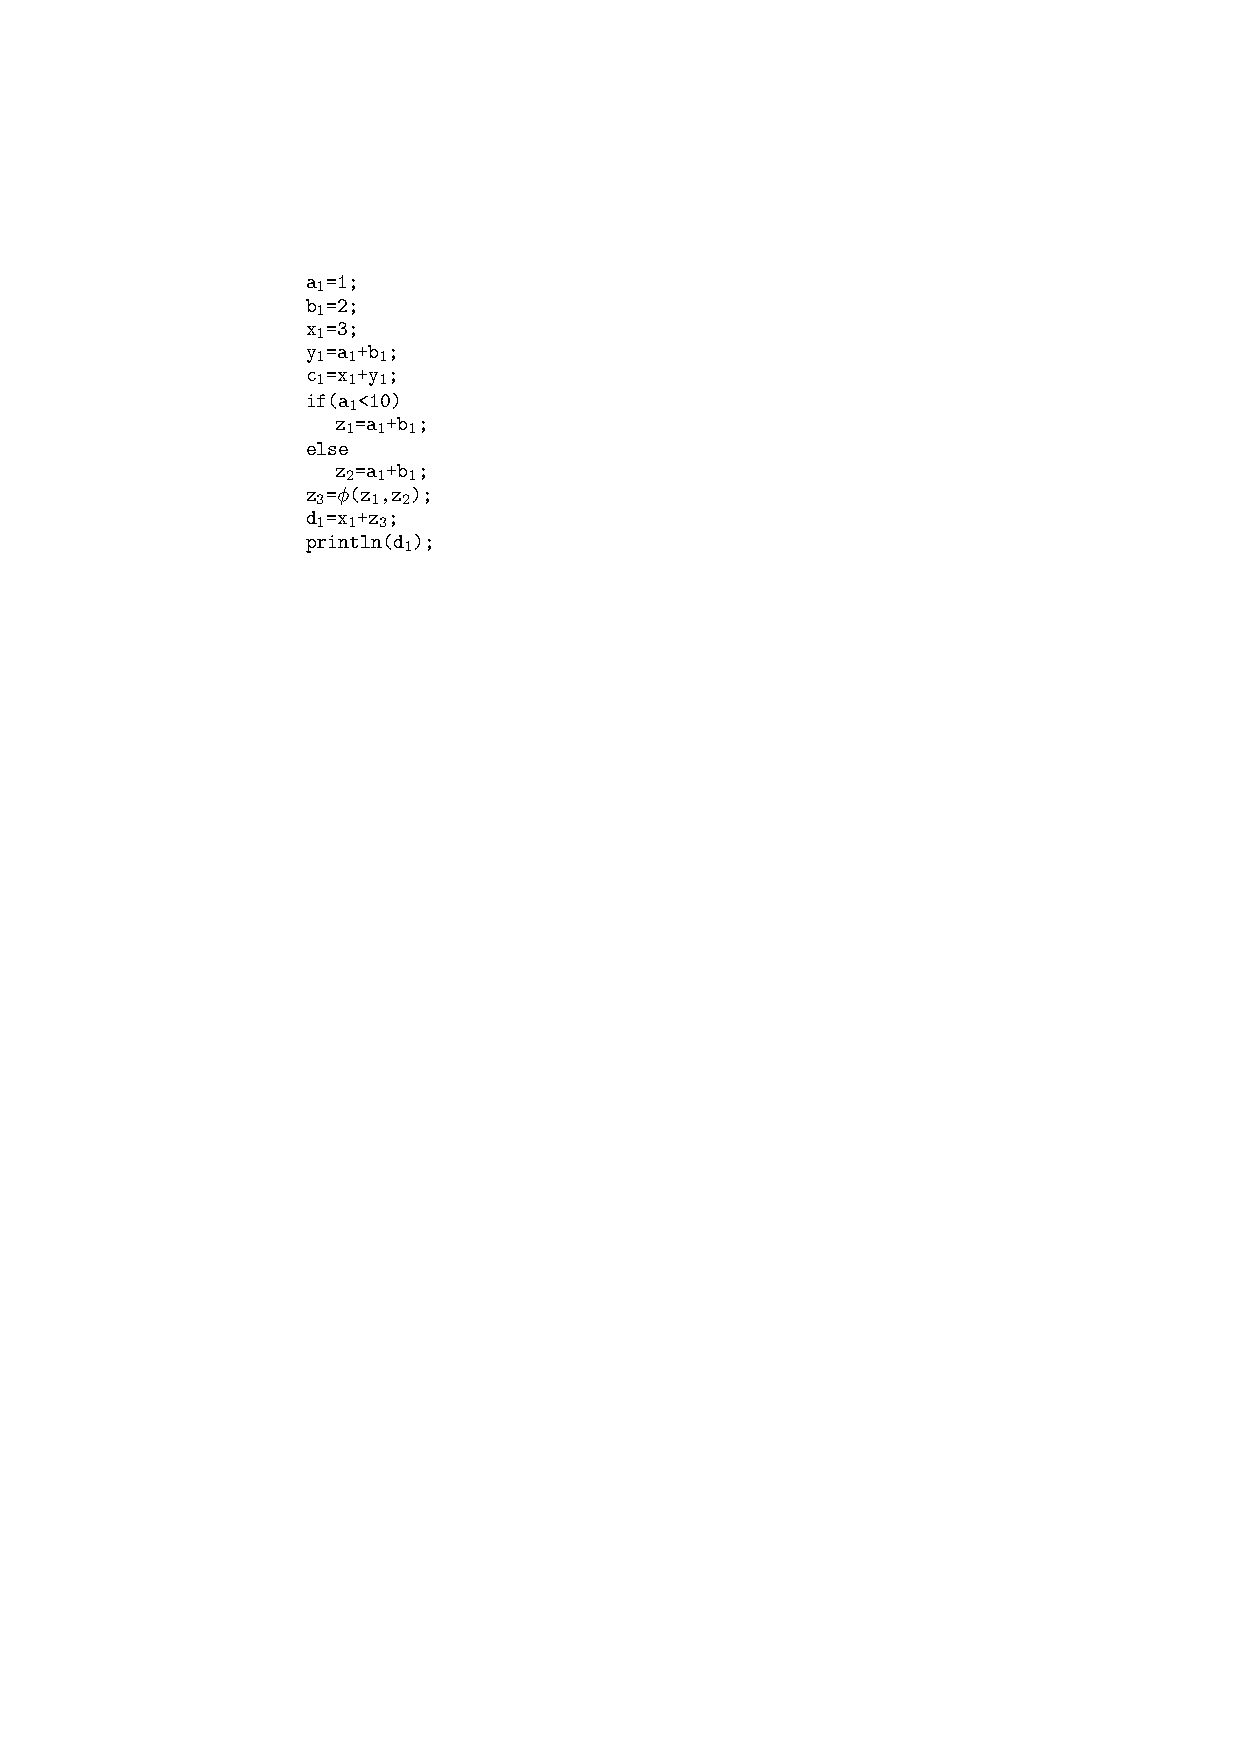
\includegraphics{ssasrc02.pdf}
%         \\[1zw]
%         \multicolumn{3}{c}{\greentext{SSA形式へ変換}}
%       \end{tabular}
%     \end{center}
%   }

%   \only<2>{
%     \begin{center}
%       \begin{tabular}{ccc}
%         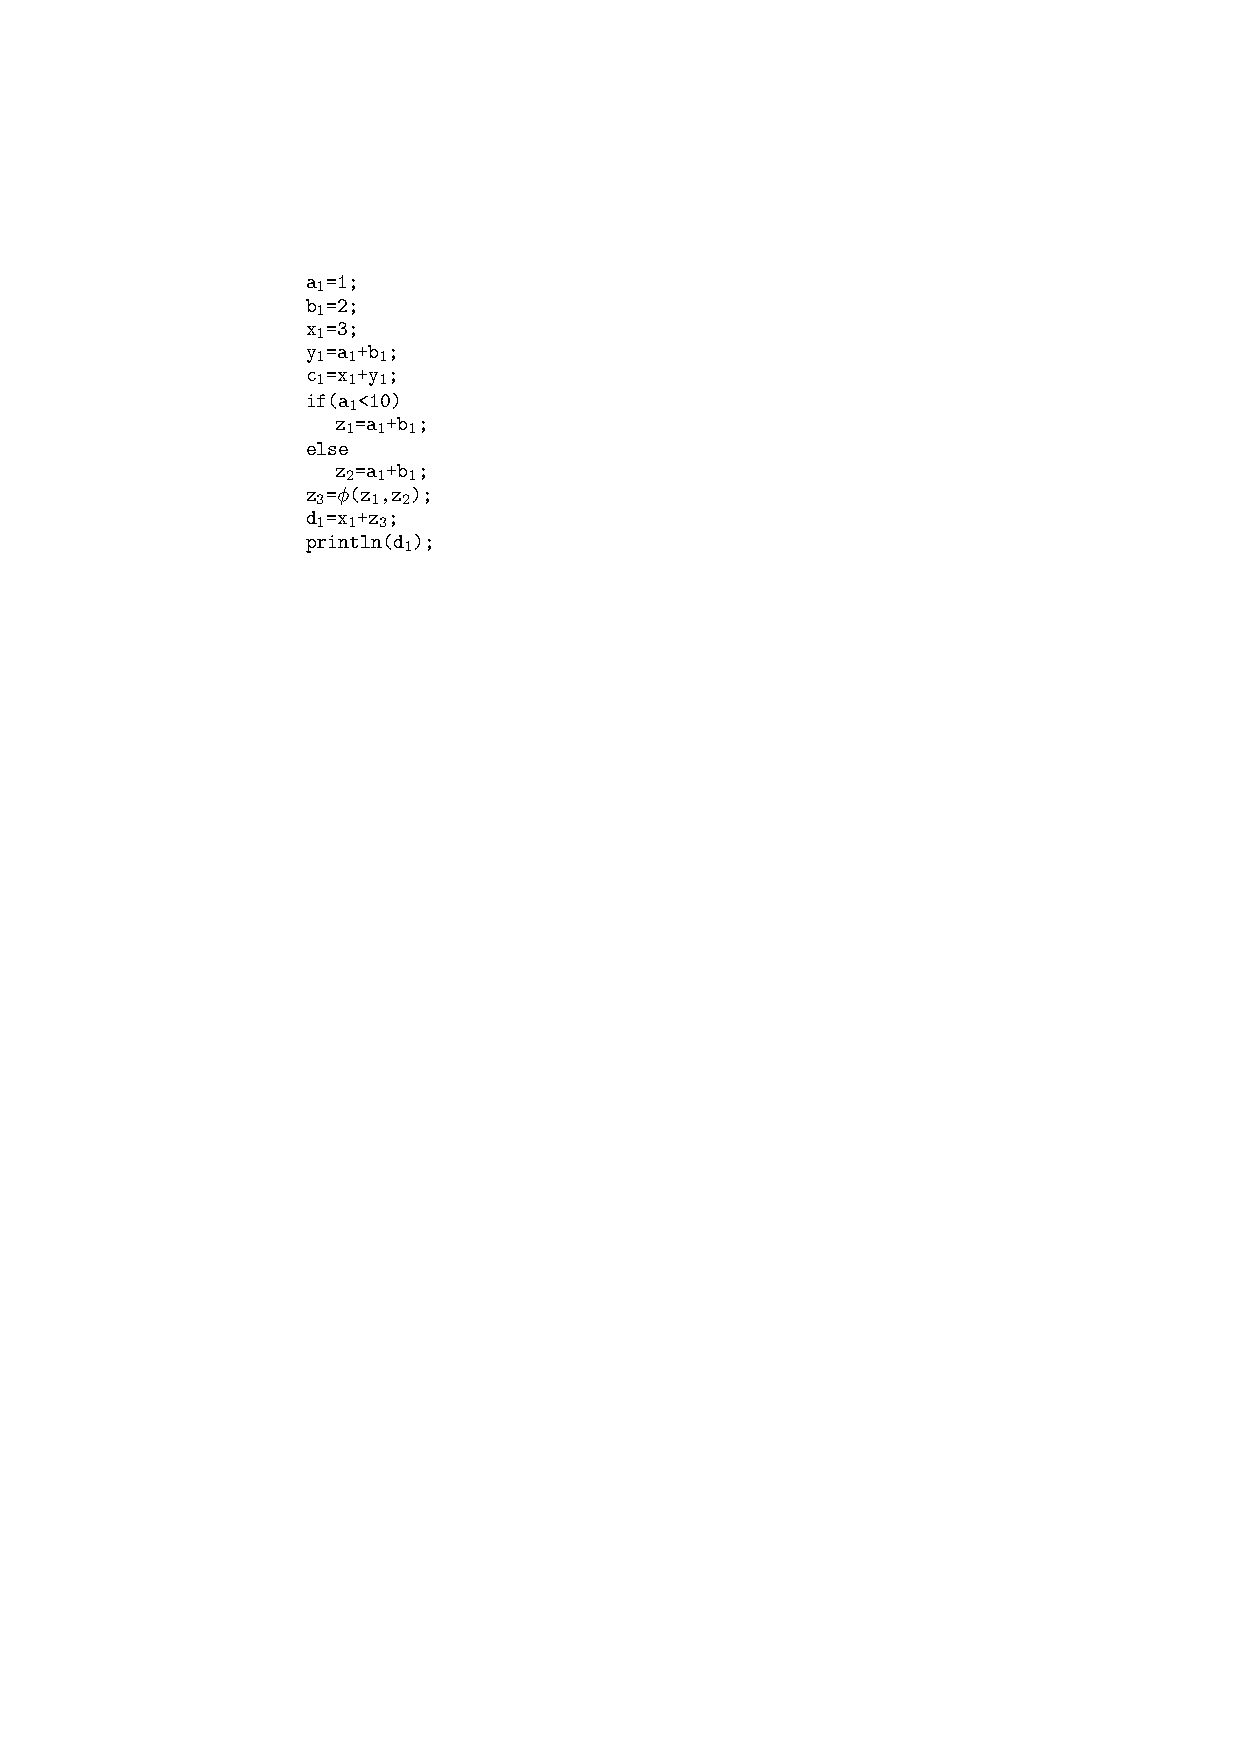
\includegraphics{ssasrc02.pdf}
%          & \hspace*{1zw}$\Rightarrow$\hspace*{1zw} &
%         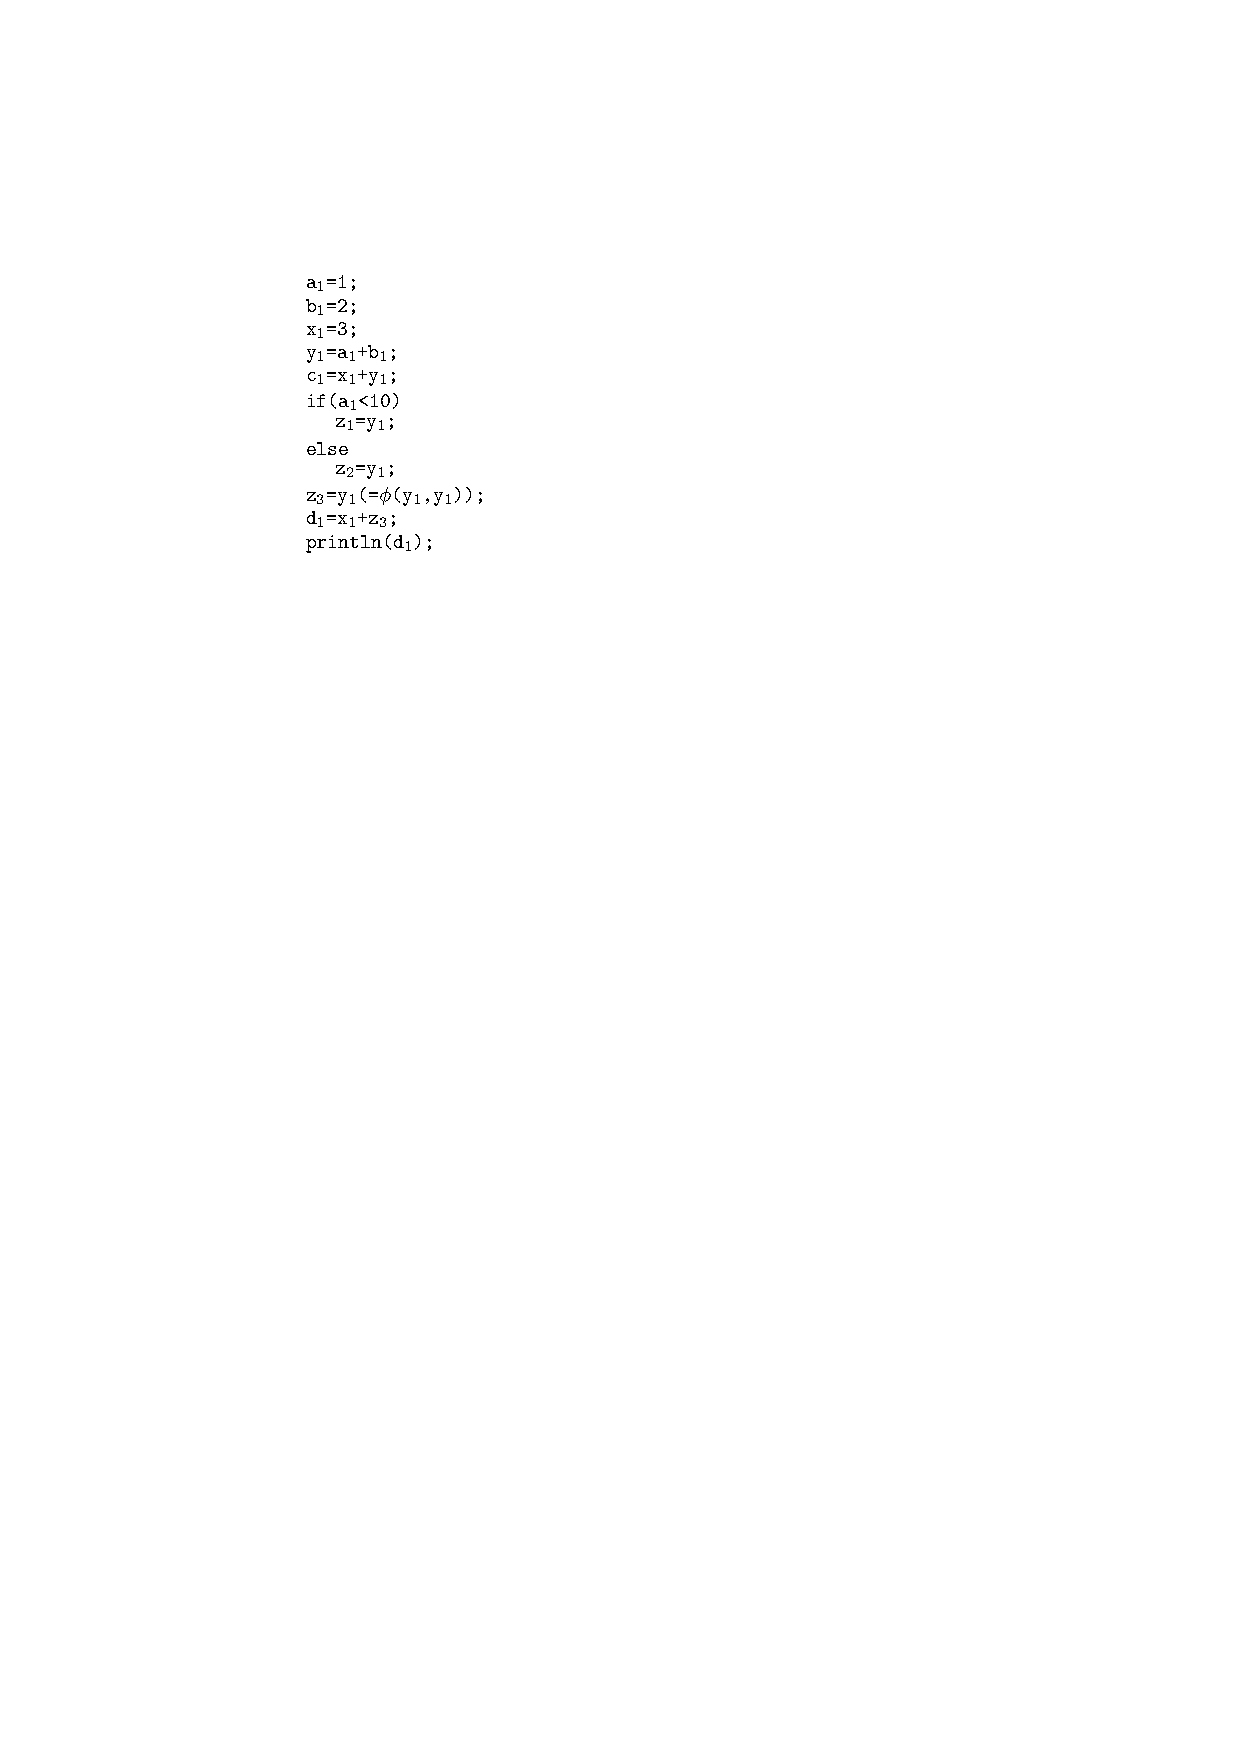
\includegraphics{ssasrc03.pdf}               \\[1zw]
%         \multicolumn{3}{c}{\greentext{共通部分式除去}}
%       \end{tabular}
%     \end{center}
%   }

%   \only<3>{
%     \begin{center}
%       \begin{tabular}{ccc}
%         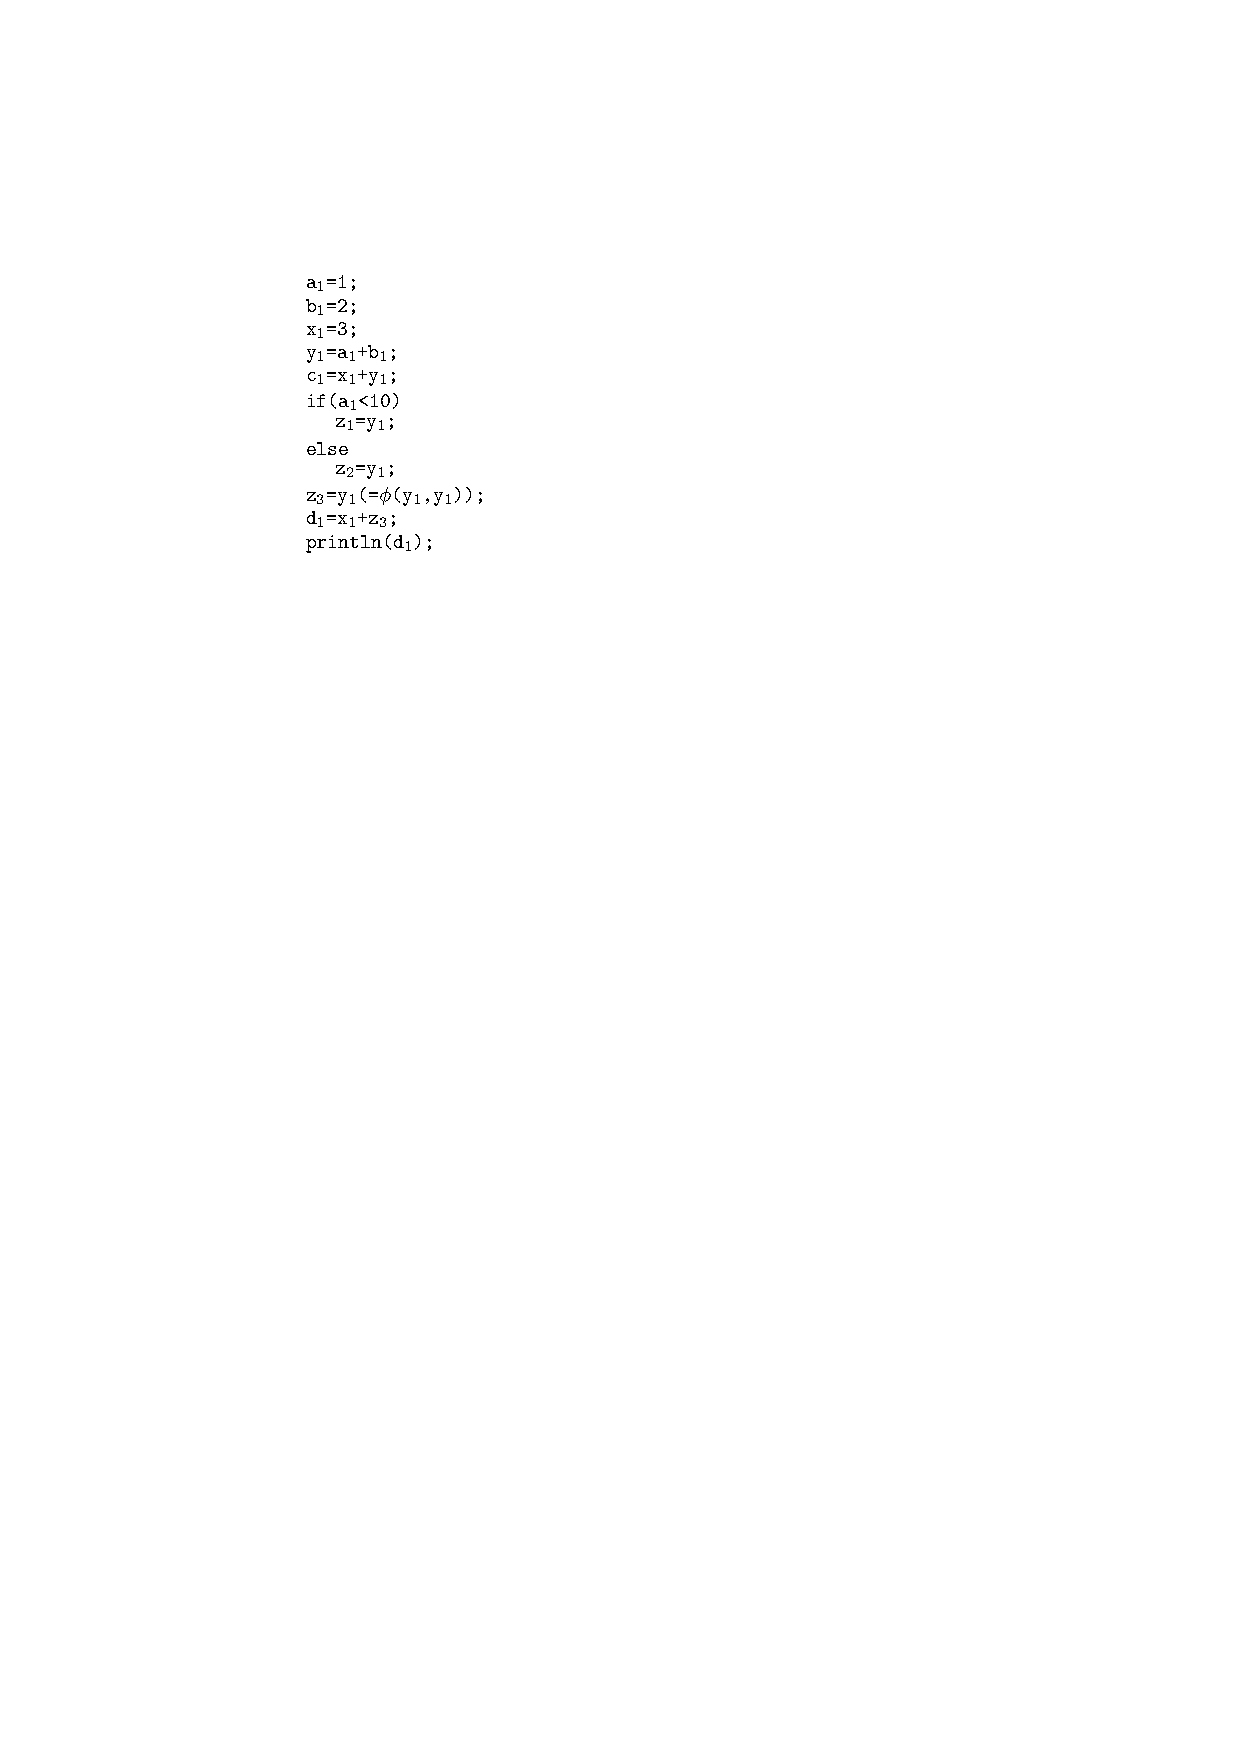
\includegraphics{ssasrc03.pdf}
%          & \hspace*{1zw}$\Rightarrow$\hspace*{1zw} &
%         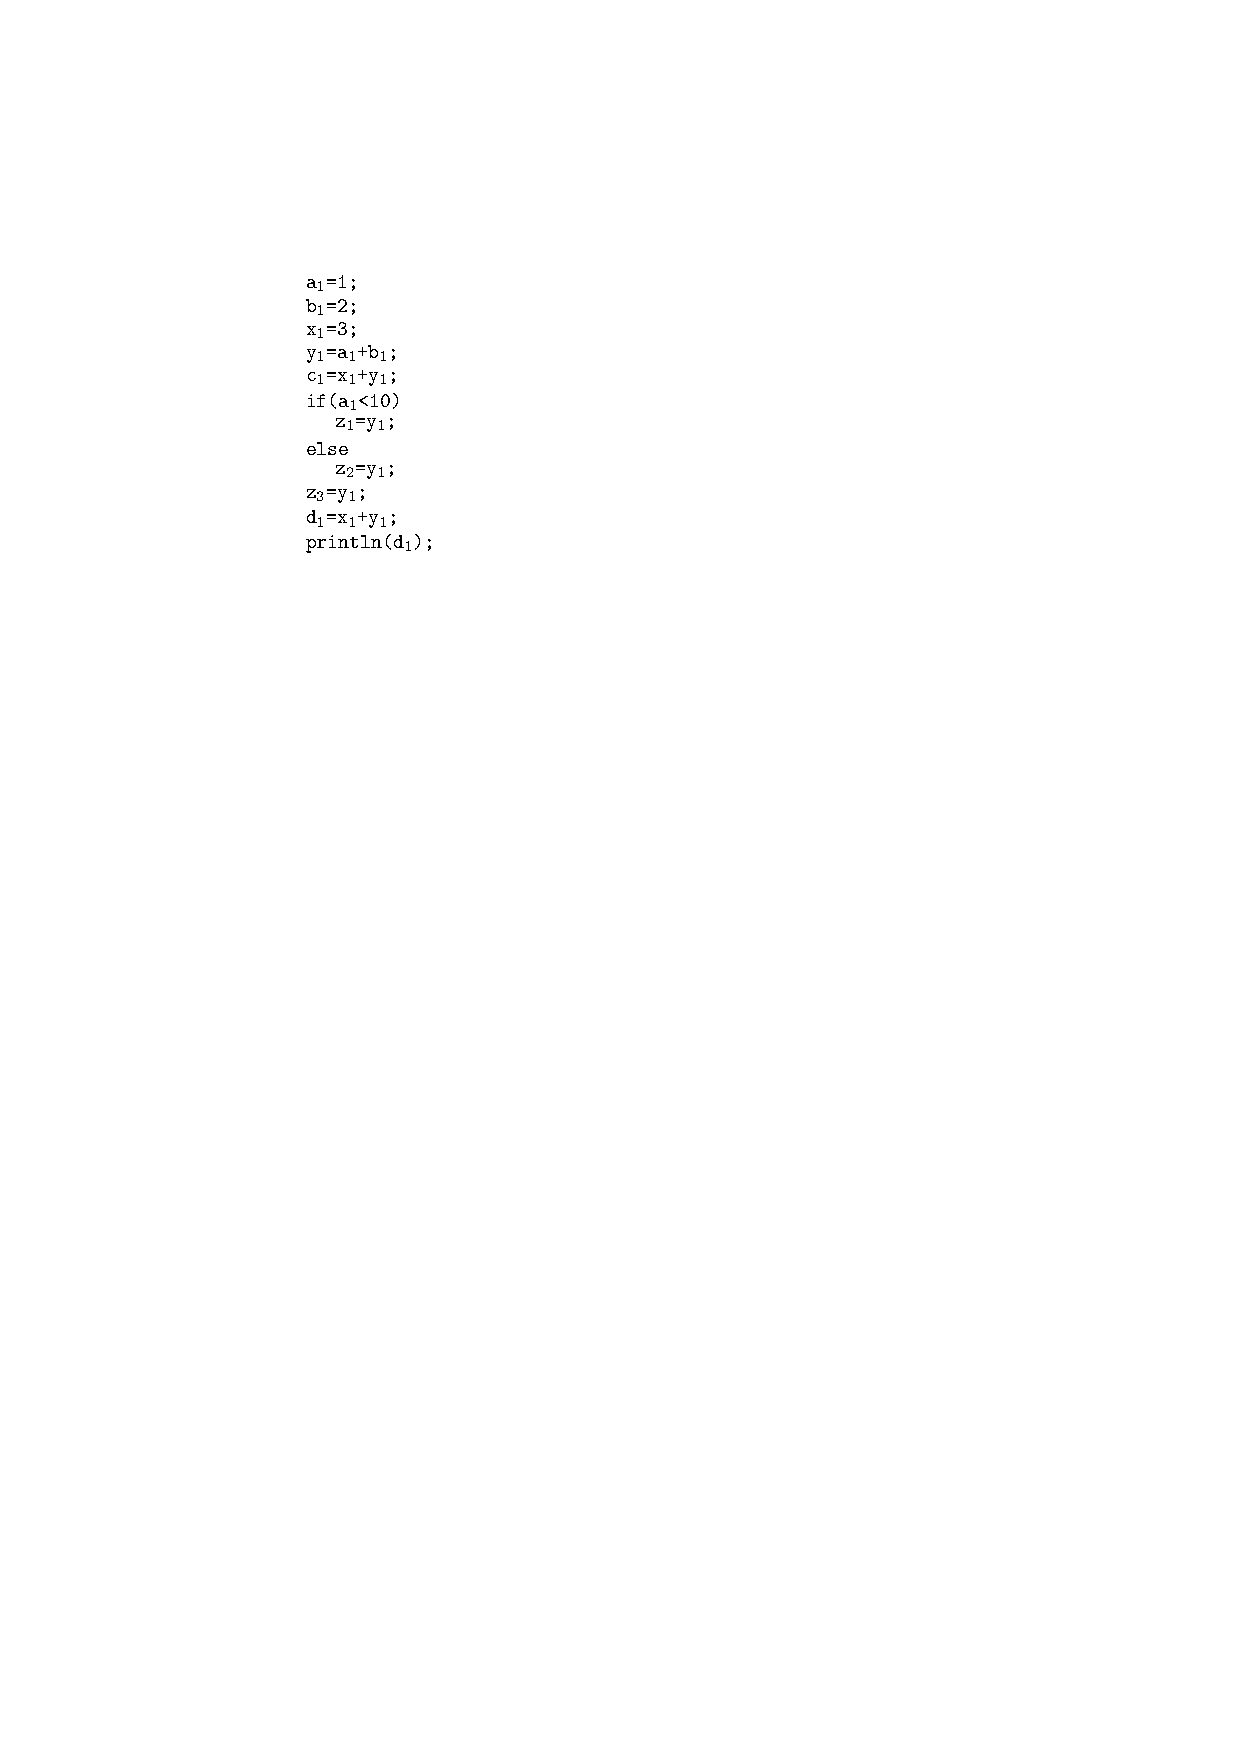
\includegraphics{ssasrc04.pdf}               \\[1zw]
%         \multicolumn{3}{c}{\greentext{コピー伝播}}
%       \end{tabular}
%     \end{center}
%   }

%   \only<4>{
%     \begin{center}
%       \begin{center}
%         \begin{tabular}{ccc}
%           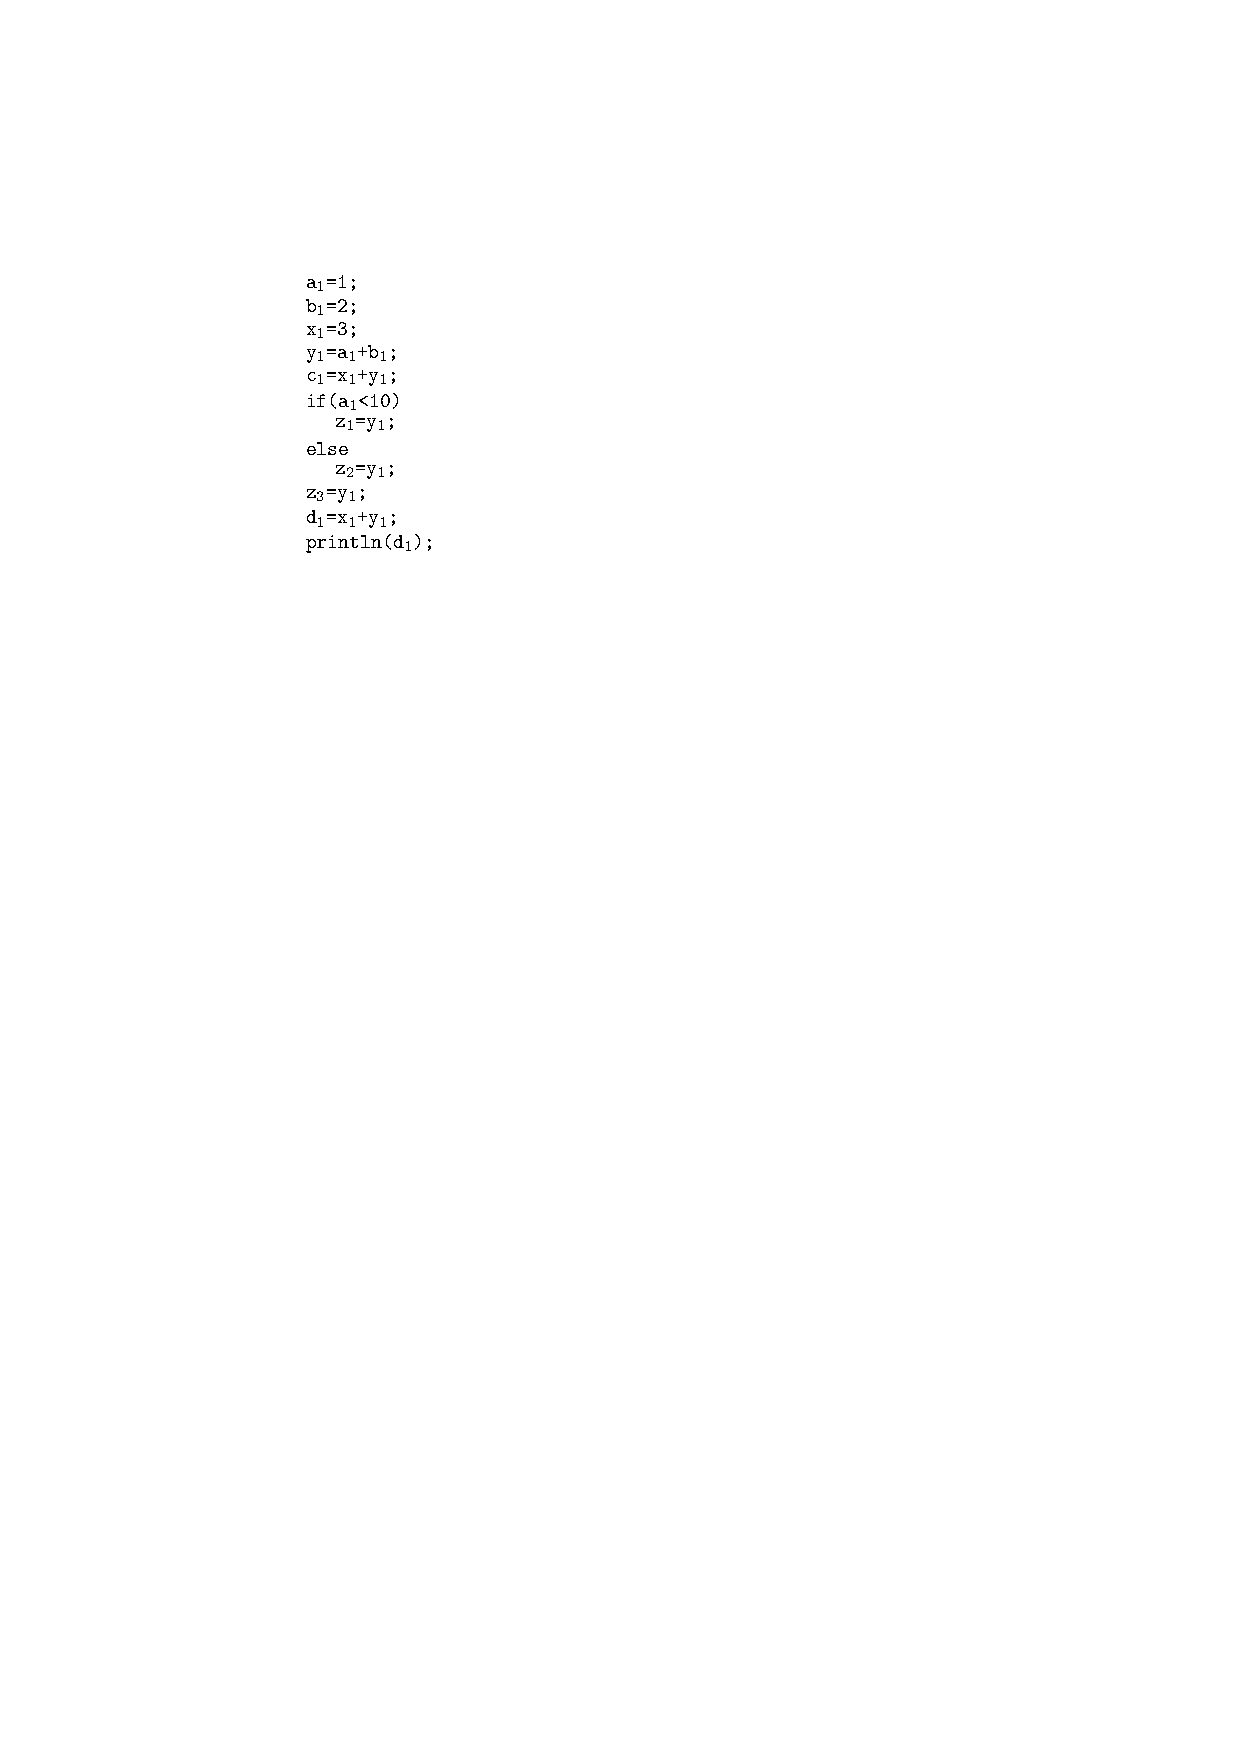
\includegraphics{ssasrc04.pdf}
%            & \hspace*{1zw}$\Rightarrow$\hspace*{1zw} &
%           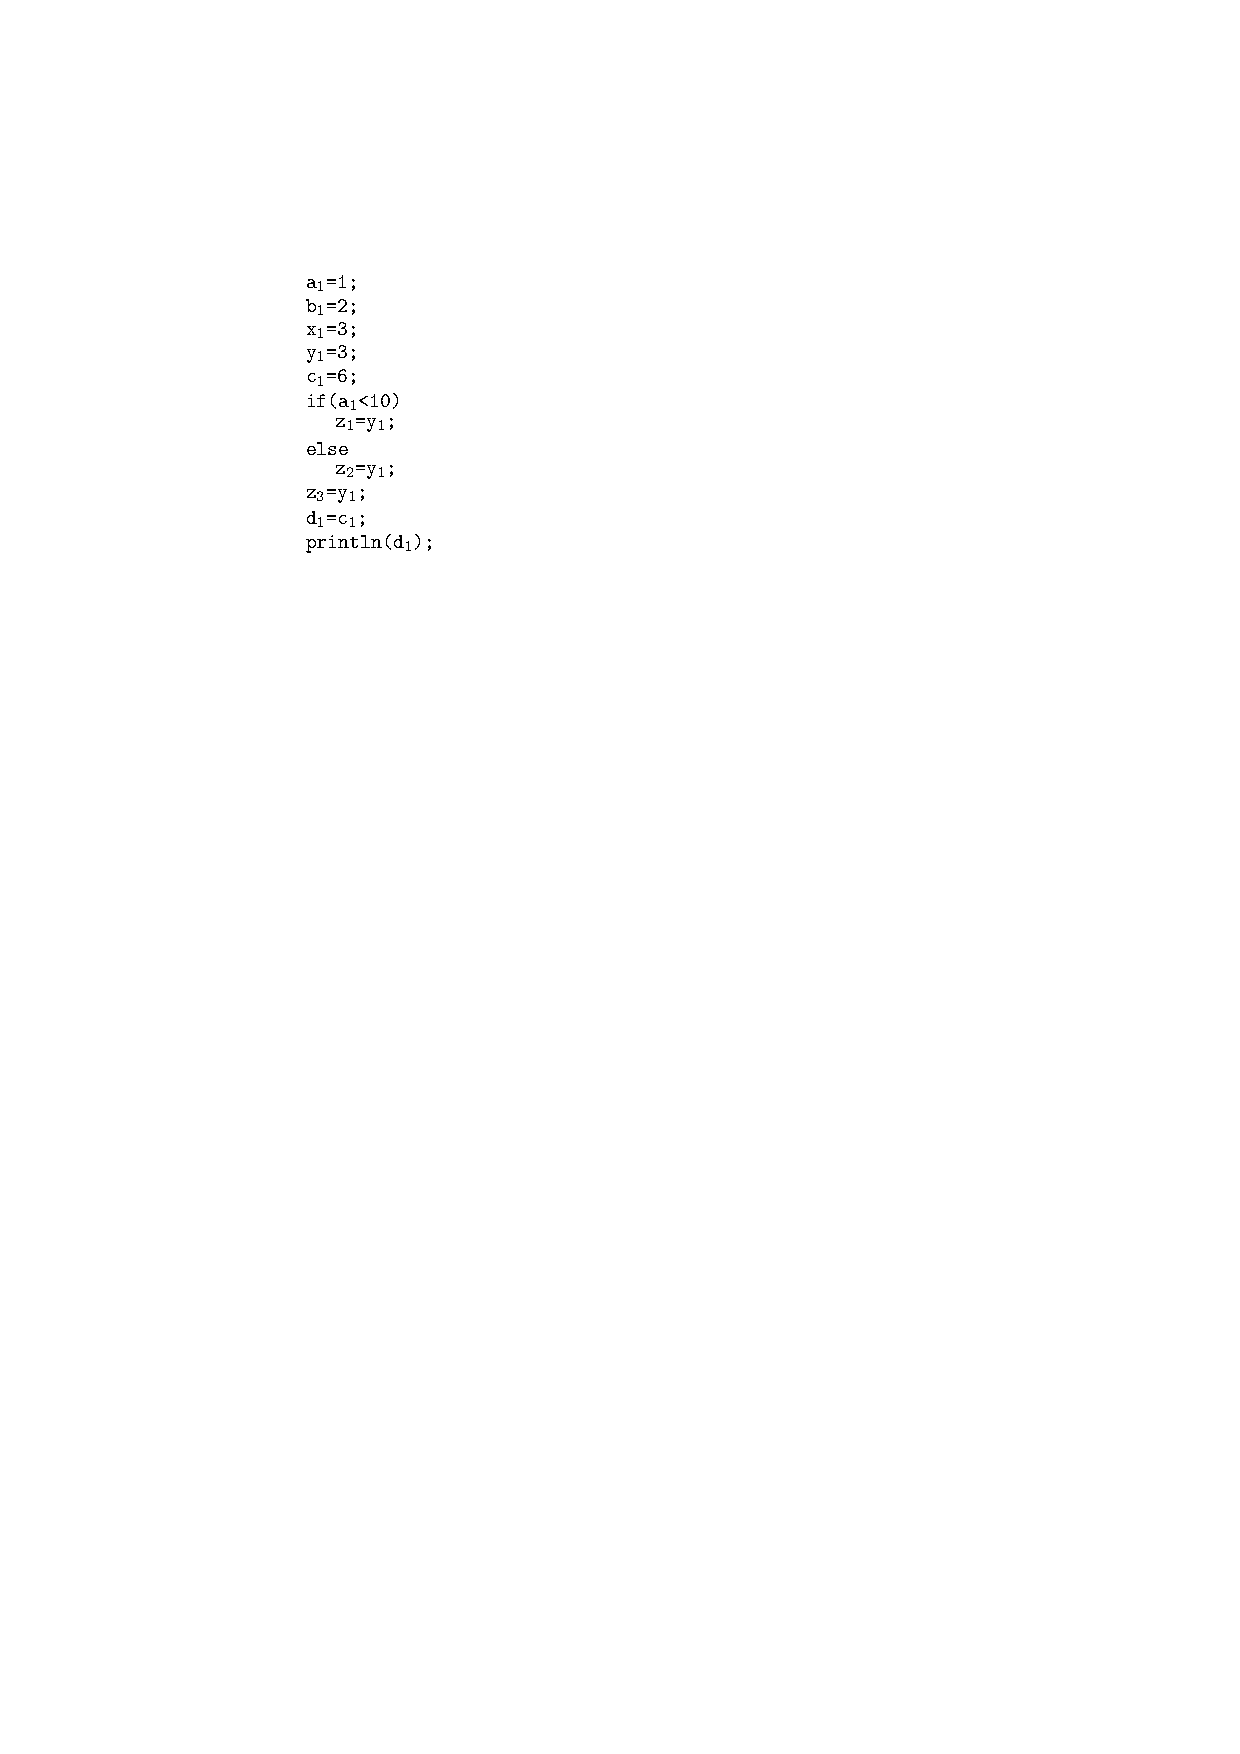
\includegraphics{ssasrc05.pdf}               \\[1zw]
%           \multicolumn{3}{c}{\greentext{共通部分式除去、定数伝播}}
%         \end{tabular}
%       \end{center}
%     \end{center}
%   }

%   \only<5>{
%     \begin{center}
%       \begin{tabular}{ccc}
%         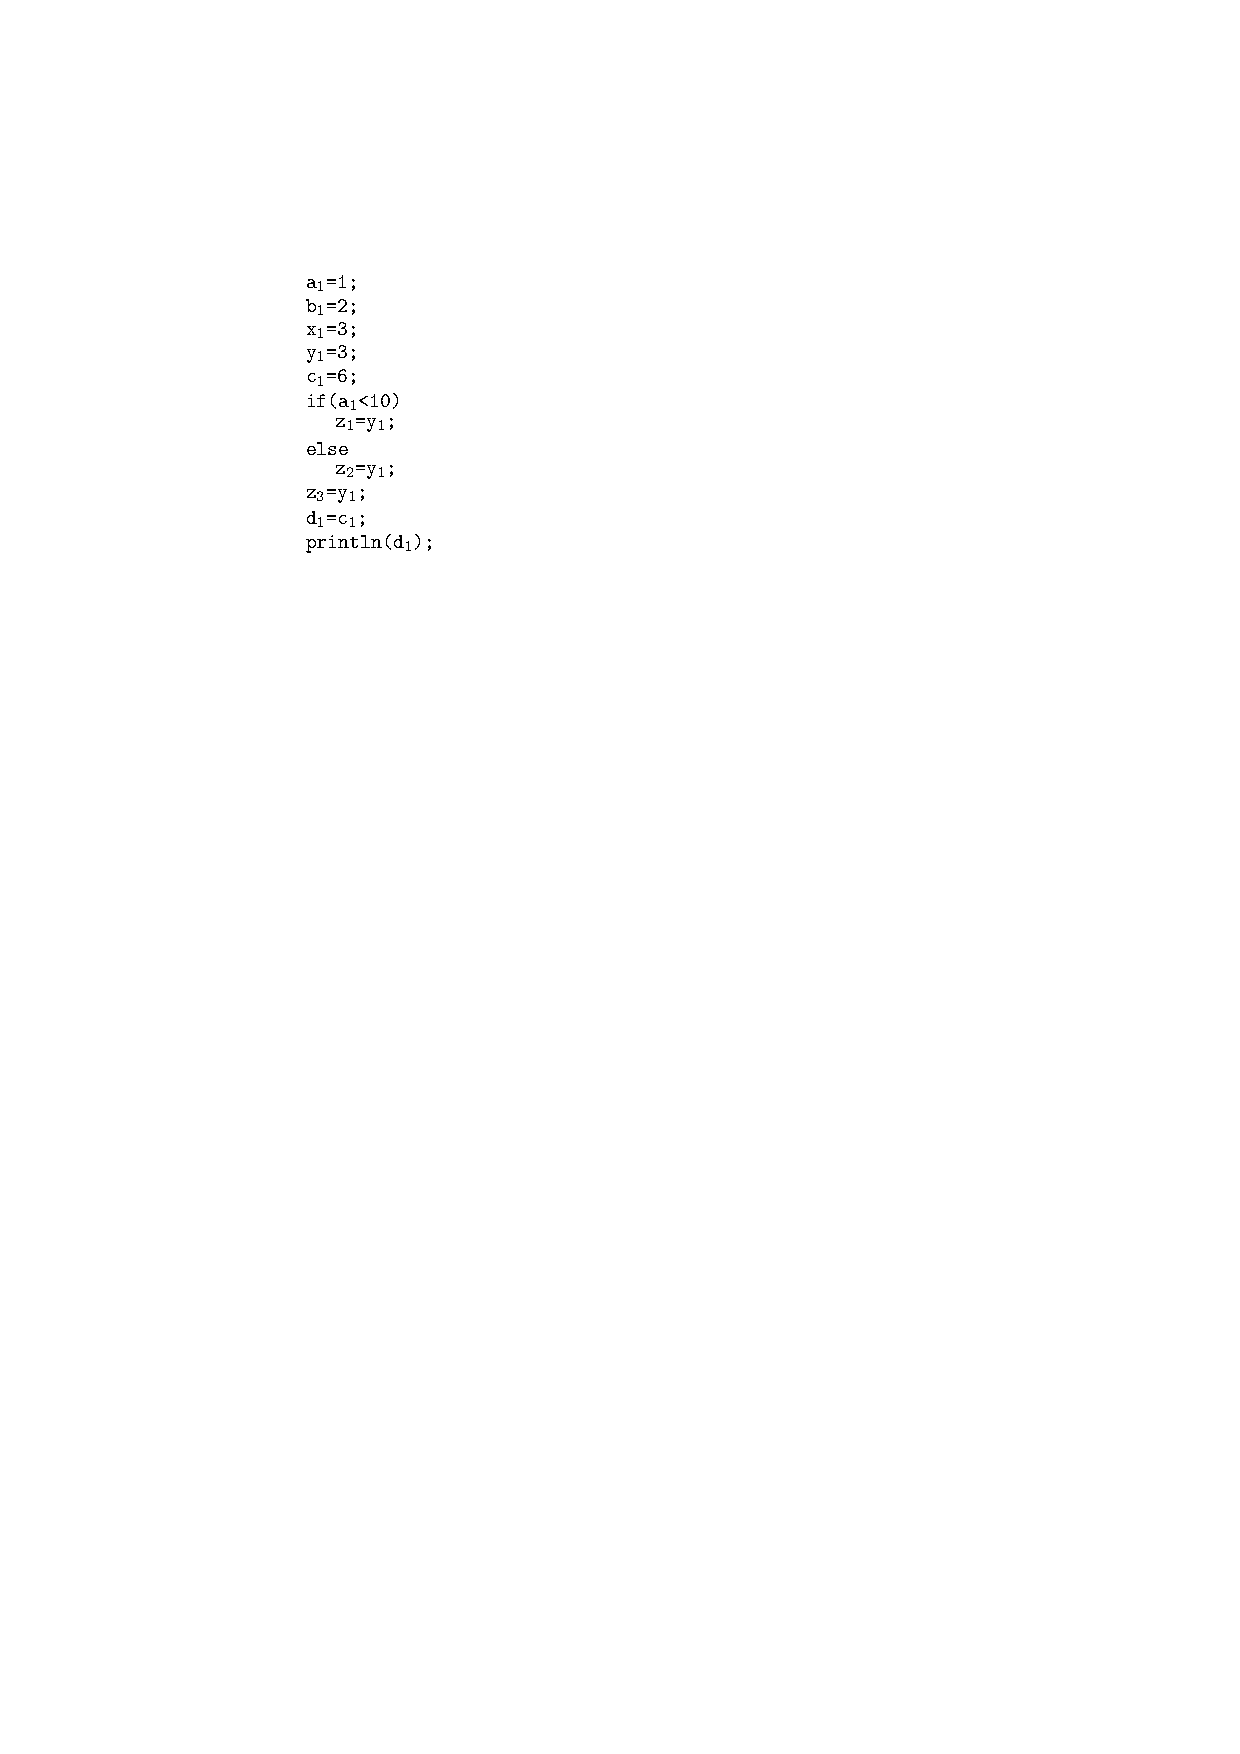
\includegraphics{ssasrc05.pdf}
%          & \hspace*{1zw}$\Rightarrow$\hspace*{1zw} &
%         
\includegraphics{ssasrc06.pdf}               \\[1zw]
%         \multicolumn{3}{c}{\greentext{コピー伝播、定数伝播、恒等式}}
%       \end{tabular}
%     \end{center}
%   }

% \end{frame}

% \begin{frame}
%   \frametitle{最適化の条件}

%   最適化を行うときに支配関係を壊さないようにする。

%   \begin{center}
%     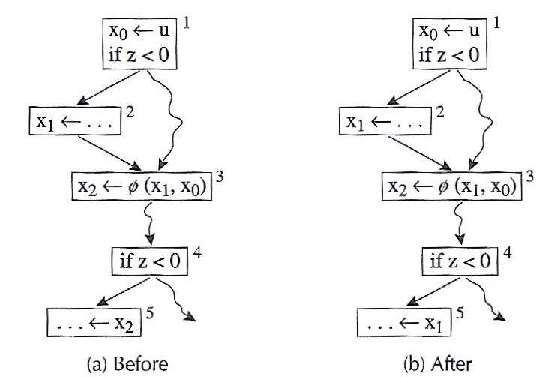
\includegraphics[height=.5\textheight]{SSAincorrectOpt.pdf}
%   \end{center}

%   $z<0$の評価は同じ方向にしかブランチしない\\
%   $\Rightarrow$ $z<0$ならば3の$\phi$関数はいつも$x_1$を$x_2$へ代入\\
%   5において$z<0$で、$x_1$を参照に用いると支配関係が壊れる\\[5pt]
%   %(支配関係を壊すと一般にはデータフローが保証されない)\\
%   厳密SSA形式：\redtext{定義が一意的＋支配関係}
%   %\greentext{静的と動的のギャップを$\phi$関数で埋めているため}
% \end{frame}

% \begin{frame}
%   \frametitle{条件付き定数伝播}
%   \begin{center}
%     {\begin{tabularx}{.75\textwidth}{XXX}
%       \multicolumn{1}{m{.35\textwidth}}{
%       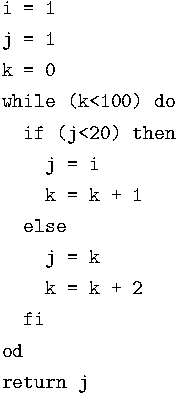
\includegraphics[height=.7\textheight]{prog-example-crop.pdf}
%       }
%       & \multicolumn{1}{m{2em}}{$\Rightarrow$} &
%       \multicolumn{1}{m{.4\textwidth}}{
%       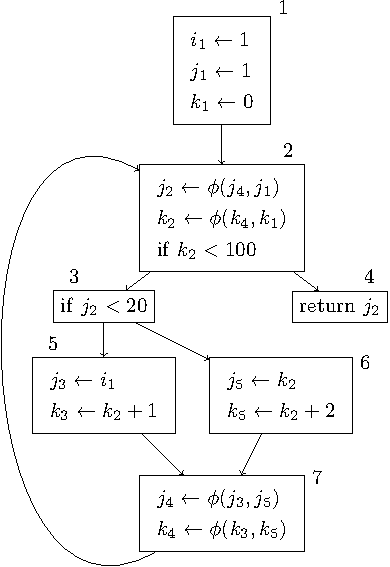
\includegraphics[height=.7\textheight]{SSA-prog-crop.pdf}
%       }
%      \end{tabularx}}
%   \end{center}
%   \centerline{\greentext{6のブロックは実行されるか？}}
% \end{frame}

% \begin{frame}
%   \frametitle{条件付き定数伝播アルゴリズム}
%   {\scriptsize
%   \begin{tabular}{l}
%   $\mathcal{B}[n]=true$ならばブロック$n$は実行される可能性あり\\
%   $\mathcal{V}[x]$ 定数$c$, 決まらない$\top$, 初期化されない$\bot$
%   \end{tabular}}

%   \vspace*{5pt}

%   {\scriptsize\color[rgb]{0,0.5,0}
%   $\phi(x_1,\ldots,x_n)$において，$x_i$のフロー元となる直近のブロックを$b_i$と書く．
%   }

%   \vspace*{5pt}

%   {\scriptsize
%   初期化：$\mathcal{B}[n]=false$ ($1\leq n\leq N$), 
%   $\mathcal{V}[x]=\bot$ ($x\in X$)
%   }

%   \vspace*{5pt}

%   {\scriptsize 
%   \begin{list}{Step \arabic{coffee}.}{\usecounter{coffee}}
%     \item 実行の引数となる変数$x\in P$について，$\mathcal{V}(x)\leftarrow\top$ 
%     \item $\mathcal{B}[1]\leftarrow true$
%   \end{list}
%   $\mathcal{B}$と$\mathcal{V}$が変化しなくなるまでStep 3 $\sim$ Step 10を繰り返す．
%   \begin{list}{Step \arabic{coffee}.}{\usecounter{coffee}\setcounter{coffee}{2}}
%     \item
%     $\mathcal{B}[n]=true$の次のブロックが唯一の$m$のとき，
%     $\mathcal{B}[m]\leftarrow true$
%     \item $z\leftarrow x\; op\; y$に対して$\mathcal{V}[x]=c_1$ かつ $\mathcal{V}[y]=c_2$
%     のとき，$\mathcal{V}[z]\leftarrow c_1\; op\; c_2$
%     \item $z\leftarrow x\; op\; y$に対して$\mathcal{V}[x]=\top$ または $\mathcal{V}[y]=\top$
%     のとき，$\mathcal{V}[z]\leftarrow\top$
%     \item $y\leftarrow\phi(x_1,\ldots,x_n)$に対して，
%     $\mathcal{V}[x_i]=c_i$, $\mathcal{V}[x_j]=c_j$, $c_i\not=c_j$となる
%     $i,j$が存在し，$\mathcal{B}[b_i]=\mathcal{B}[b_j]=true$のとき，$y\leftarrow\top$
%     \item $y\leftarrow\phi(x_1,\ldots,x_n)$に対して，
%     $\mathcal{V}[x_i]=\top$となる$i$が存在するならば$\mathcal{V}[y]=\top$
%     \item $y\leftarrow\phi(x_1,\ldots,x_n)$に対して，
%     $\mathcal{B}[b_i]=true$である$x_i$ですべて$\mathcal{V}[x_i]=c$であり，
%     $\mathcal{B}[b_j]=false$である$x_j$ですべて$\mathcal{V}[x_j]=\bot$ならば，
%     $\mathcal{V}[y]\leftarrow c$
%     \item $\mathbf{if}\ x<y\ \mathbf{goto}\ B_i\ \mathbf{else}\ B_j$に対して
%     $\mathcal{V}[x]=\top$ または $\mathcal{V}[y]=\top$ならば
%     $\mathcal{B}[i]\leftarrow true$, $\mathcal{B}[j]\leftarrow true$
%     \item $\mathbf{if}\ x<y\ \mathbf{goto}\ B_i\ \mathbf{else}\ B_j$に対して
%     $\mathcal{V}[x]=c_1$, $\mathcal{V}[y]=c_2$のとき，$c_1<c_2$ならば
%     $\mathcal{B}[i]\leftarrow true$, $c_1\not<c_2$ならば$\mathcal{B}[j]\leftarrow true$.
%   \end{list}
%   }

% \end{frame}

% \begin{frame}
% \frametitle{条件付き定数伝播}

% \begin{center}
%   \begin{tabularx}{.6\textwidth}{cc}
%     \multicolumn{1}{m{.3\textwidth}}{
%      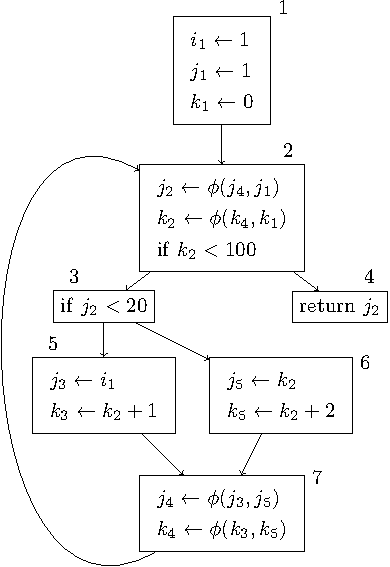
\includegraphics[width=.3\textwidth]{SSA-prog-crop.pdf}
%      }
%      &
%      {\small
%      \begin{tabularx}{0.3\textwidth}{XXXXX}
%        $B$ & $\mathcal{E}[B]$ & & $x$ & $\mathcal{V}[x]$\\\cline{1-2}\cline{4-5}
%        1 & $true$ & & $i_1$ & $1$\\
%        2 & $true$ & & $j_1$ & $1$\\
%        3 & $true$ & & $j_2$ & $1$\\
%        4 & $true$ & & $j_3$ & $1$\\
%        5 & $true$ & & $j_4$ & $1$\\
%        6 & $false$ & & $j_5$ & $\bot$\\
%        7 & $true$ & & $k_1$ & $0$\\
%          &        & & $k_2$ & $\top$\\
%          &        & & $k_3$ & $\top$\\
%          &        & & $k_4$ & $\top$\\
%          &        & & $k_5$ & $\bot$
%      \end{tabularx}}
%    \end{tabularx}
%    \end{center}
%    \greentext{$j$は定数が伝播して，$j<20$の判定がいつも成立．$k$は$\top$なので$k<100$の
%    判定は実行時}
% \end{frame}

% \begin{frame}
%   \frametitle{条件付き定数伝播}
%   \begin{center}
%     \begin{tabularx}{0.8\textwidth}{XXX}
%       \multicolumn{1}{m{.3\textwidth}}{
%         \only<1>{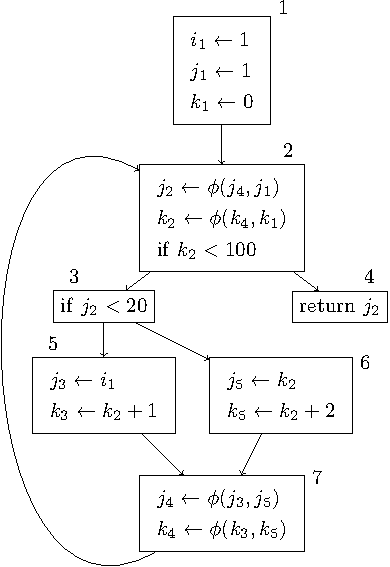
\includegraphics[width=.3\textwidth]{SSA-prog-crop.pdf}}
%         \only<2>{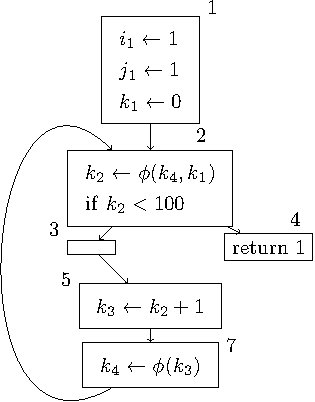
\includegraphics[width=.3\textwidth]{SSA-prog-opt1-crop.pdf}}
%       }
%       &
%       \multicolumn{1}{m{2em}}{$\Rightarrow$} 
%       &
%       \multicolumn{1}{m{.3\textwidth}}
%       {
%         \only<1>{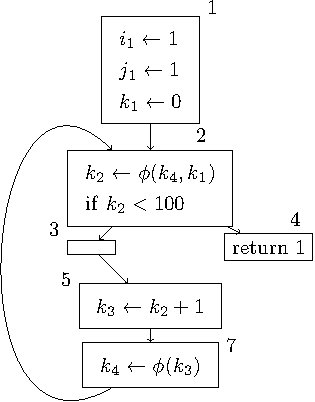
\includegraphics[width=.3\textwidth]{SSA-prog-opt1-crop.pdf}}
%         \only<2>{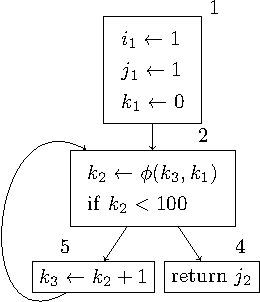
\includegraphics[width=.3\textwidth]{SSA-prog-opt2-crop.pdf}}
%       }
%     \end{tabularx}
%   \end{center}
% \end{frame}

\end{document}
